
% Bug: automatically loads natbib with name options, cannot be
% overridden, `Elsevier LaTeX' style produces error messages

\documentclass[review]{elsarticle}
%\documentclass{elsarticle}

\usepackage{hyperref}
\usepackage{lineno,hyperref} \modulolinenumbers[5]
\usepackage{graphicx}
\usepackage{mathtools}
\usepackage{units}
\usepackage[ruled,vlined]{algorithm2e}
\usepackage{physics} % normal derivative v=dv{x}{t},
                     % partial derivative pdv{V(x,t)}{t}
                     % n'th normal derivative a=dv[2]{x}{t}


\usepackage{color}
\providecommand{\red}[1]{\textcolor{red}{#1}}
\providecommand{\blue}[1]{\textcolor{blue}{#1}}
\definecolor{green}{rgb}{0,0.7,0}
\providecommand{\green}[1]{\textcolor{green}{#1}}

% local macros

\providecommand{\martin}[1]{\red{#1}} %literal, Preprint
\providecommand{\martinc}[1]{\green{[#1]}} %comment, Preprint
%\providecommand{\martin}[1]{#1}                  %fuer Veroeffentlichung
%\providecommand{\martinc}[1]{#1}                  %fuer Veroeffentlichung

\providecommand{\sup}[1]{^{\mathrm{#1}}}  % upright superscript
\providecommand{\sub}[1]{_{\mathrm{#1}}}  % upright subscript $b\sub{comf}$
                                        % symbolic subscripts without:
                                        % $\epsilon_t$
\providecommand{\3}{{\ss}}

\journal{Transportation Research Part C}

%%%%%%%%%%%%%%%%%%%%%%%
%% Elsevier bibliography styles
%%%%%%%%%%%%%%%%%%%%%%%
%% To change the style, put a % in front of the second line of the current style and
%% remove the % from the second line of the style you would like to use.
%%%%%%%%%%%%%%%%%%%%%%%

%% Numbered
\bibliographystyle{model1-num-names}

%% Numbered without titles
%\bibliographystyle{model1a-num-names}
 
%% Harvard
%\bibliographystyle{model2-names.bst}\biboptions{authoryear}

%% Vancouver numbered
%\usepackage{numcompress}\bibliographystyle{model3-num-names}

%% Vancouver name/year
%\usepackage{numcompress}\bibliographystyle{model4-names}\biboptions{authoryear}

%% APA style
%\bibliographystyle{model5-names}\biboptions{authoryear}

%% AMA style
%\usepackage{numcompress}\bibliographystyle{model6-num-names}

%% `Elsevier LaTeX' style
% \bibliographystyle{elsarticle-num}
%%%%%%%%%%%%%%%%%%%%%%%

\begin{document}

\begin{frontmatter}

\title{Formulation and validation of a car-following model based on deep
  reinforcement learning}

%% Group authors per affiliation:
%\author{Fabian Hart\fnref{myfootnote}}
%\address{TU Dresden}
%\fntext[myfootnote]{Comment.}

%% or include affiliations in footnotes:
\author[firstAddress]{Fabian Hart}
\author[firstAddress,secondAddress]{Ostap Okhrin}
\author[firstAddress,secondAddress]{Martin Treiber\corref{corrAuthor}}
\cortext[corrAuthor]{Corresponding author}
\ead{Martin.treiber@tu-dresden.de}
\ead[url]{www.mtreiber.de}

\address[firstAddress]{TU Dresden}
\address[secondAddress]{Possible second address}




\begin{abstract}
To be written at the end
\end{abstract}

\begin{keyword}
reinforcement learning \sep car-following model \sep stochastic
processes \sep string stability \sep validation \sep trajectory data 
\end{keyword}

\end{frontmatter}

%\linenumbers

\section{Introduction}

Autonomous driving technologies are seen as promising solutions to improve road safety, where human errors account for 94\% of the total accidents \cite{vehicleCrashSurvey2015}. Moreover congestion, energy consumption and emissions are intended to be reduced. 
But autonomous driving is a challenging task since the transportation traffic can be dynamic and unpredictable.
On the way to fully autonomous driving, Advanced Driver Assistance Systems
(ADAS) has been developed to solve tasks like lane-keeping, lane-changing, car-following, emergency braking, etc.
Since Deep Learning methods has been demonstrated to surpass humans in certain domains, they are also adopted in the area of autonomous driving.
Especially Deep Reinforcement Learning (DRL), which combines the power of Deep Learning in tackling large, complicated problems with Reinforcement Learning, has shown its potential in a broad variety of autonomous driving tasks. 
In \cite{OnRampMerge2018} and \cite{OnRampMerge2020}, DRL is used to guide an autonomous vehicle safely from on-ramp to freeway. In \cite{intersection1}, \cite{intersection3} and \cite{intersection2}, DRL methods are used to manage traffic of autonomous vehicles at intersections, optimizing safety and efficiency.
In \cite{LangeChange1}, DRL is used to solve lane change maneuvers.

A further task in autonomous driving is to model the vehicle behavior under car following scenarios, where suitable accelerations has to computed in order to achieve a safe and comfortable driving. Approaches to solve this task are classical car-following models, such as the Intelligent Driver Model \cite{Opus} or stochastic car-following models, such as in \cite{Treiber2018stochIDM_TRB}. Furthermore data-driven approaches use Machine Learning methods to train a car-following model based on experimental car-follower data, such as in \cite{Chong2011SimulationOD} or \cite{ZHOU2017245}. Downside of this approach is that the model tries to emulate human driver behavior which still can be suboptimal.

To overcome this issue, DRL methods train non-human car-following models that can optimize metrics such as safety, efficiency and comfort. 
One approach is to train on scenarios, where the leading vehicle trajectory, used for training, is based on experimental data, such as in \cite{SafeEfficientAndComfortable} or \cite{HumanLikeAutonomouCF}. Similar approaches suggest a standardized driving cycle, which functions as leading vehicle trajectory, such as \cite{ComparisonRLvsMPC} or \cite{CFelectricVehicle}, which uses the New European Driving Cycle.
A disadvantage coming along with these approaches is, that for scenarios, which are not in the scope of the training data, the performance decreases, indicating inadequate machine learning generalization \cite{ComparisonRLvsMPC}. 

Another issue of car-following models is string-stability. There are several studies focusing on dampening traffic oscillations by using a sequence of trained vehicles, such as \cite{qu2020jointly}, \cite{DissipatingStopAndGoWaves} and \cite{DampenStopAndGoTraffic}.

All the mentioned DRL car-following models have three disadvantages in common: At first the acceleration range is limited in a way, that full-brakes are not considered. This results in models that are just designed for non-safety-critical scenarios. Second these models just consider car-following scenarios, while free driving or the transition between both is not reflected in the reward function. Third the trained models have just been validated on data that is similar to the training data set, so that the generalization capabilities cannot be proved. 

This motivated us to design a model, which overcomes these issues.
To our knowledge, no RL based car-following model has been proposed which has the following features combined:


\begin{itemize}
	\item  The proposed model considers free driving, car-following, as well as the transition between both in a way, that approaching of the leading vehicle is smooth and comfortable.
	\item The proposed model has a wider range of possible accelerations, which leads to a collision-free behavior also in safety-critical situations such as full-braking of the leader.
	\item The proposed model is trained on leading trajectories, based on an AR(1)-process, e. g. \cite{HonerkampEngl}, the parameters reflecting kinematics of real drivers. This leads to high generalization capabilities and a model usage in a broader variety of traffic scenarios. 
	\item Different driver characteristics can be modeled by adjusting the parameters of the reward function.
	\item The proposed model shows string-stability.
	
\end{itemize}

Another feature of this work is a thorough validation of the above mentioned properties in scenarios based on both synthetic and naturalistic trajectory data, bringing the model to its limits. 
In all cases, the model proved to be accident free and string stable.
In a further experiment the proposed model is compared to an Intelligent Driver Model, calibrated on the same data. The results indicate a better performance of the proposed model.


[short textual enumeration of the sections to come]

\section{Reinforcement Learning Background}
The following vehicle is controlled by a Reinforcement
Learning (RL) agent. By interaction with an environment, the RL agent
optimizes a sequential decision making problem. At each time step
$t$, the agent observes an environment state $s_t$ and, based on that state, selects
an action $a_t$. After conducting action $a_t$, the RL agent receives
a reward $r(a_t,s_t)$. The agent aims to learn an optimal state-action
mapping policy $\pi$ that maximizes the expected accumulated
discounted reward
\begin{equation}
\label{Rt}
R_{t}=\sum_{k=0}^{\infty} \gamma^{k} r_{t+k},
\end{equation}
 where $\gamma = (0,1]$ denotes the discount factor and 
$\gamma^k r_{t+k}$ the expected contribution $k$ time steps ahead. 
  \subsection{\label{RL-algorithm}RL algorithm}
  In various similar control problems, the Deep Deterministic Policy
  Gradient (DDPG) Algorithm has been used and proven to perform well on
  tasks with a continuous action and state space, such as in
  \cite{SafeEfficientAndComfortable}, \cite{ComparisonRLvsMPC} or
  \cite{HumanLikeAutonomouCF}. The original work can be found in
  \cite{DDPG}. DDPG is an Actor-Critic method, that uses an Actor  $\mu\left(s \mid \theta^{\mu}\right)$ with weights $\theta^{\mu} $ to propose an action based on a given state $s$ and a Critic $Q\left(s, a \mid \theta^{Q}\right) $ with weights  $\theta^{Q}$ to predict if the action is good or bad, based on a given state $s$ and action $a$. To achieve a better training stability, DDPG uses target networks  $\mu^{\prime}$ and $Q^{\prime}$ for Actor and Critic. While training, these networks are updated slowly, hence keeping the estimated targets stable. Furthermore DDPG uses Experience Replay, that implements a Replay Buffer $R$, where a list of tuples $\left(s_{t}, a_{t}, r_{t}, s_{t+1}\right)$ are stored. Instead of learning from the most recent experience, DDPG learns from sampling a mini-batch from the experience buffer. To implement better exploration by the Actor network, DDPG uses noisy perturbations, specifically an Ornstein-Uhlenbeck process for generating noise. It samples noise from a correlated normal distribution. The entire DDPG algorithm is shown in Algorithm~\ref{alg:ddpg}. 
  
  \begin{algorithm}
  	\label{alg:ddpg}
  	Randomly initialize critic network $Q\left(s, a \mid \theta^{Q}\right) $ and actor $\mu\left(s \mid \theta^{\mu}\right)$ with weights $\theta^{Q}$ and $\theta^{\mu} $  \\
  	Initialize target network $Q^{\prime}$ and $\mu^{\prime}$ with weights $\theta^{Q^{\prime}} \leftarrow \theta^{Q}, \theta^{\mu^{\prime}} \leftarrow \theta^{\mu}$\\
  	Initialize Replay Buffer $R$\\
  	\For{$episode = 1$ \KwTo $M$}{
  		Initialize a random process $\mathcal{N}$ for action exploration\\
  		 Receive initial observation state $s_{1}$ \\
  		\For{$t = 1$ \KwTo $T$}{
  			Select action $a_{t}=\mu\left(s_{t} \mid \theta^{\mu}\right)+\mathcal{N}_{t}$ according to the current policy and exploration noise\\
  			 Execute action $a_{t}$ and observe reward $r_{t}$ and observe new state $s_{t+1}$\\
  			  Store transition $\left(s_{t}, a_{t}, r_{t}, s_{t+1}\right)$ in $R$\\
  			   Sample a random minibatch of $N$ transitions $\left(s_{i}, a_{i}, r_{i}, s_{i+1}\right)$ from $R$\\
  			    Set $y_{i}=r_{i}+\gamma Q^{\prime}\left(s_{i+1}, \mu^{\prime}\left(s_{i+1} \mid \theta^{\mu^{\prime}}\right) \mid \theta^{Q^{\prime}}\right)$\\
  			Update critic by minimizing the loss: $L=\frac{1}{N} \sum_{i}\left(y_{i}-Q\left(s_{i}, a_{i} \mid \theta^{Q}\right)\right)^{2}$\\
  			 Update the actor policy using the sampled policy gradient:
  			$$
  			\left.\left.\nabla_{\theta^{\mu}} J \approx \frac{1}{N} \sum_{i} \nabla_{a} Q\left(s, a \mid \theta^{Q}\right)\right|_{s=s_{i}, a=\mu\left(s_{i}\right)} \nabla_{\theta^{\mu}} \mu\left(s \mid \theta^{\mu}\right)\right|_{s_{i}}
  			$$
  			Update the target networks:
  			$$
  			\begin{aligned}
  			\theta^{Q^{\prime}} & \leftarrow \tau \theta^{Q}+(1-\tau) \theta^{Q^{\prime}} \\
  			\theta^{\mu^{\prime}} & \leftarrow \tau \theta^{\mu}+(1-\tau) \theta^{\mu^{\prime}}
  			\end{aligned}
  			$$
  		}
  	}
  	
  	
  	\caption{DDPG algorithm according to \cite{DDPG}}
  \end{algorithm}
  
  
  \subsection{\label{MRL}Modularized Reinforcement Learning}
  Furthermore we used a modularized approach to decompose the task into two subtasks. Modular Reinforcement Learning (MRL) refers to the decomposition of a complex, multi-goal
  problem into a collection of simultaneously running single goal learning processes, typically modeled as Markov Decision Processes. Typically, these subagents share an action
  set but have their own reward signal and state space. At each
  time step, every subagent reports a numerical preference for
  each available action to an arbitrator, which then selects one
  of the actions for the agent as a whole to take (\cite{MRL}). There are numerous works, that are using a modularized Reinforcement Learning approach, like in \cite{MRLexample1}, \cite{MRLexample2} or \cite{MRLexample3} to name just a few. The advantage of decomposing multiple-goal reward functions with MRL, we also want to use in this work. 
  Figure \ref{fig:MRL} shows the architecture of our MRL System. We divide our car-following problem into two subtasks, handled by two different policies. The Free-Driving-Policy refers to free driving and aims to not to exceed a desired speed. The Car-Following-Policy refers to following a vehicle and aims to keep a reasonable gap to a leader vehicle. Although both policies are trained with different reward functions and in different training environments, they both output an acceleration value. As an arbitrator between both accelerations we use a simple min-function. In the next sections the model specifications of the Free-Driving-Policy and the Car-Following-Policy, which are both trained with the DDPG algorithm, are described in detail.
  
  \begin{figure}
  	\centering
  	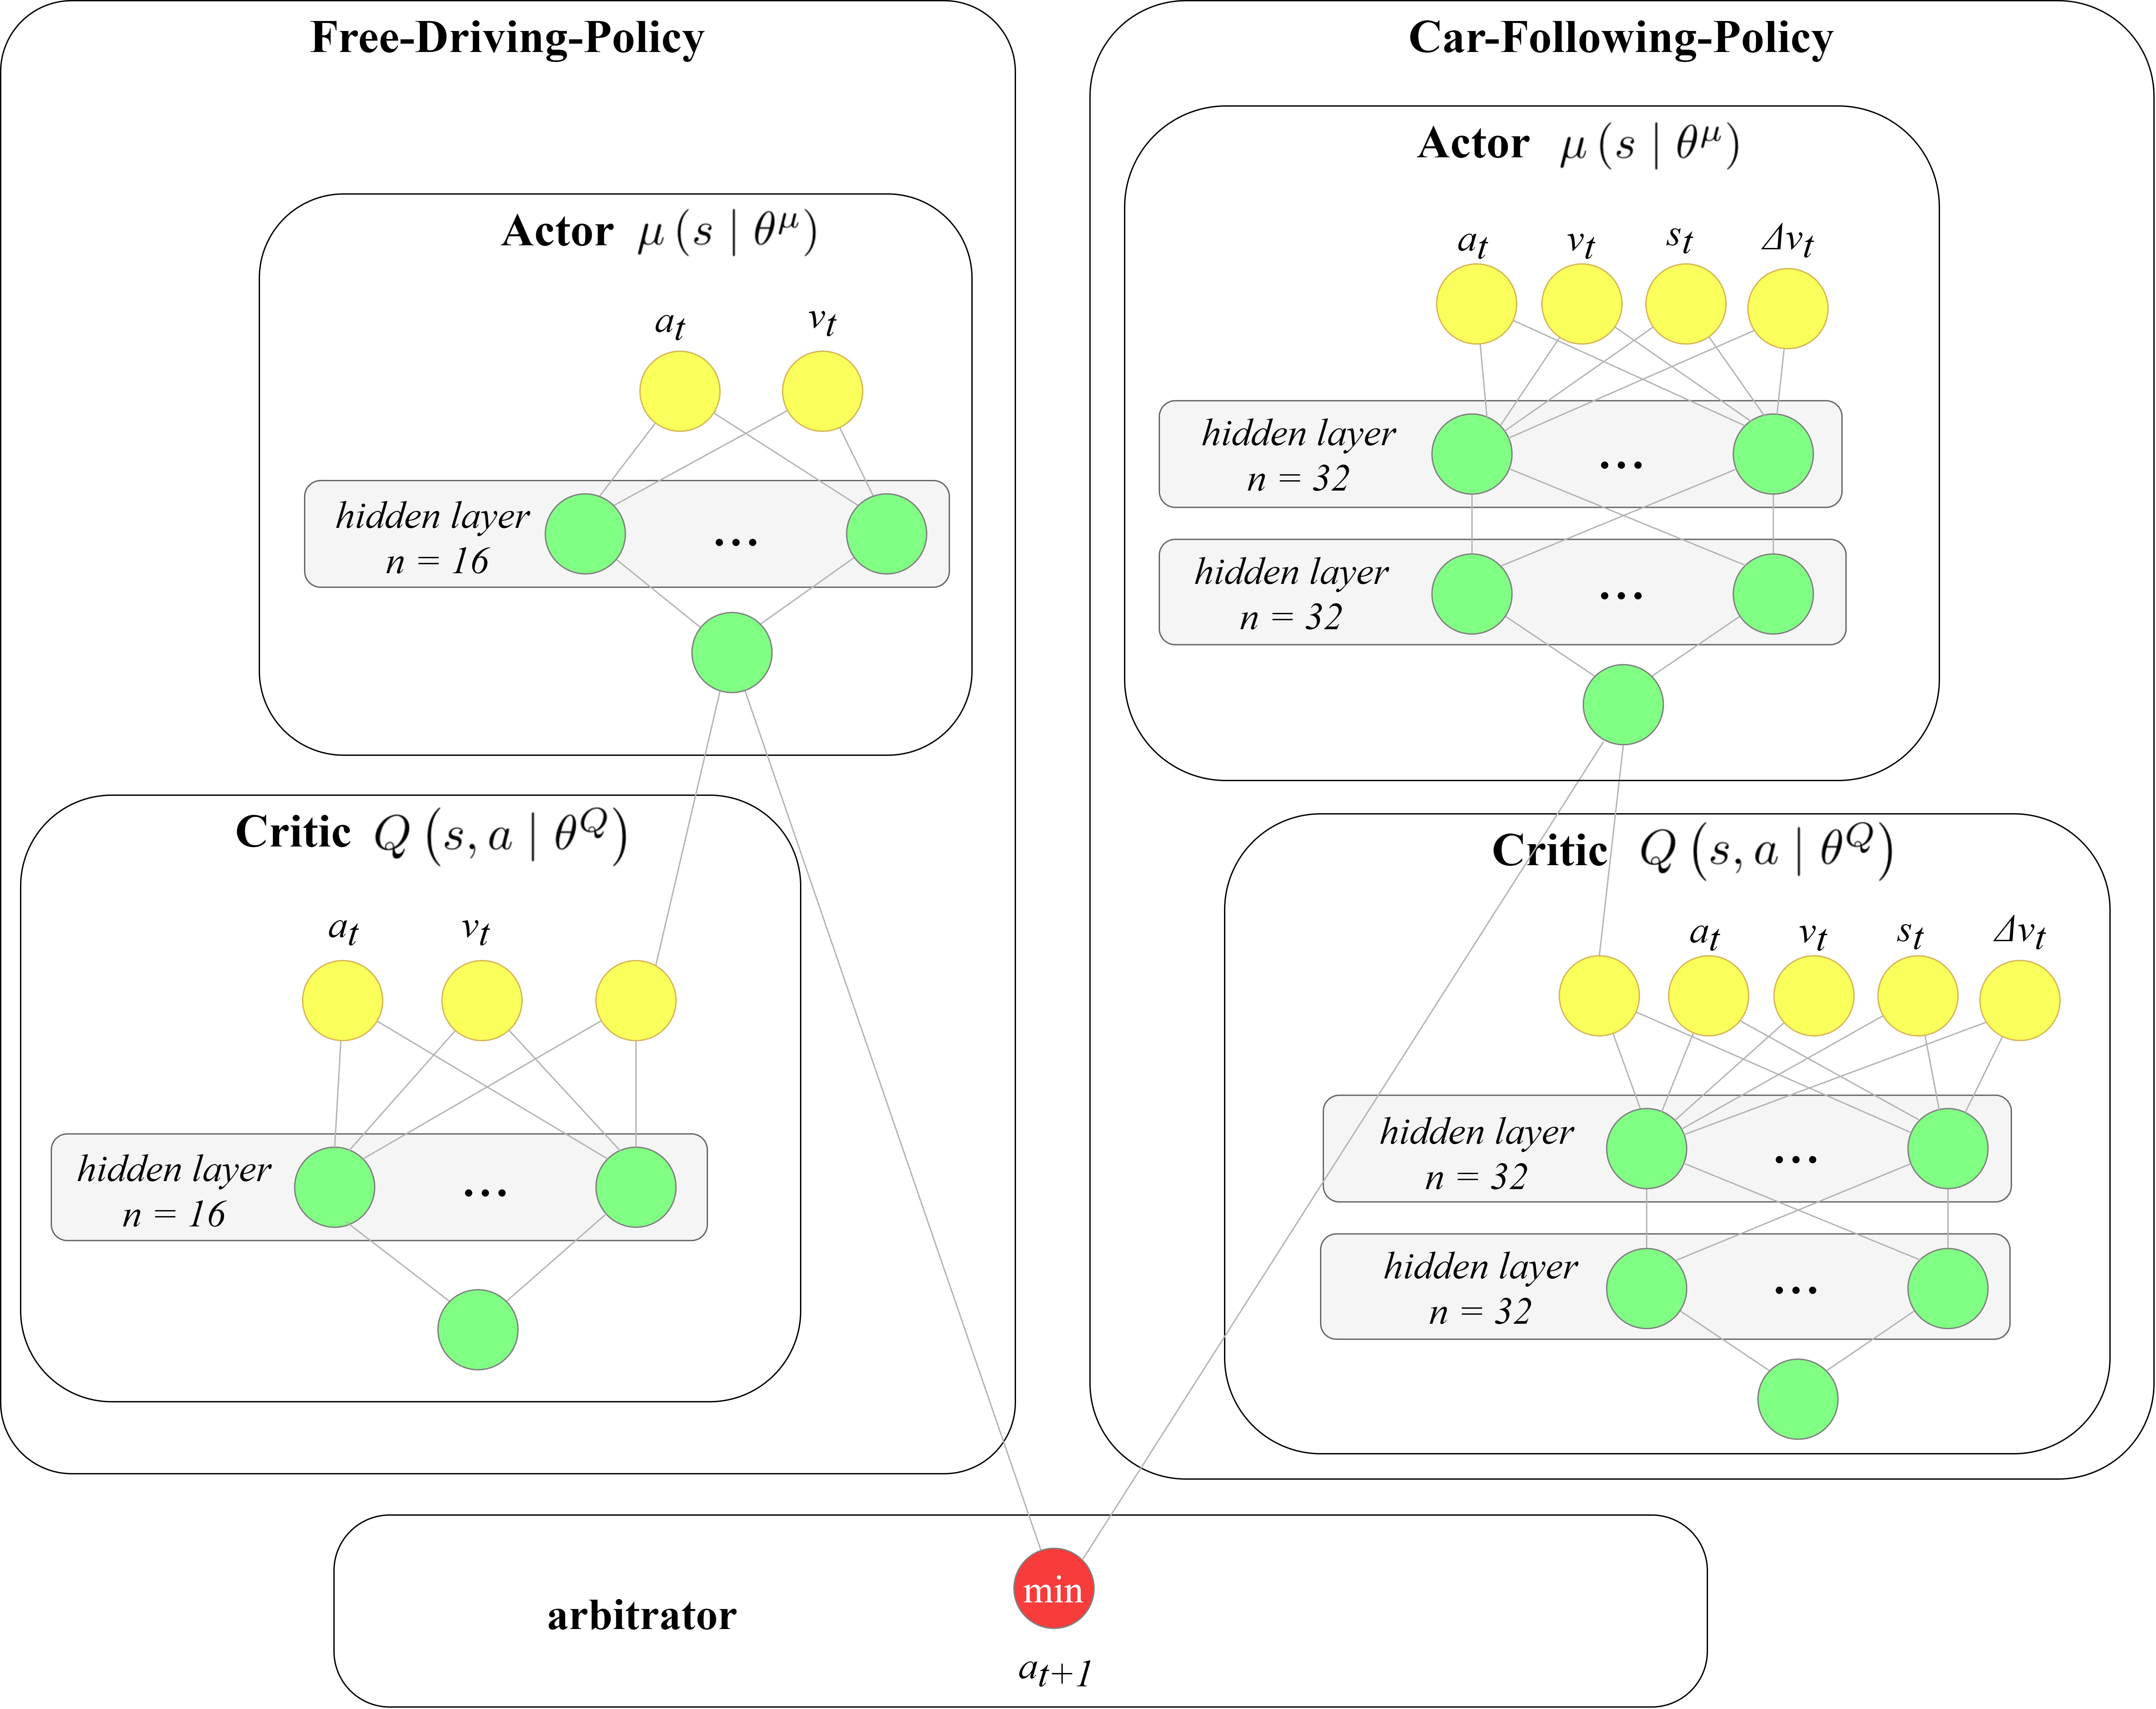
\includegraphics[width=12cm]{images/MRL}
  	\caption{Modularized RL architecture with actor networks of both policies.} 
  	\label{fig:MRL}
  \end{figure}

  
  % In this study, both networks are feed-forward neural networks with two layers of hidden neurons and %32 neurons each hidden layer. All DDPG parameters are presented in Table \ref{tab:DDPGparameters}.
  



\section{Free-Driving-Policy}
\subsection{Action and state space}
\label{actionSpace1}
 The defined modularized RL approach requires that the action space of both sub-policies are identical. To enable comfortable driving and allow for a maximum braking deceleration in safety-critical
situations, the acceleration is defined as a continuous variable in the
  range between $a\sub{\rm min} = \unit[-9]{m/s^2}$ and $a\sub{\rm max} =\unit[2]{m/s^2}$.

%\martinc{In contrast to variables or symbolic
%    constants which are set in italic, units are set in roman
%    (upright) font. If super- or subscripts are variables, they are
%    set italic. If they are abbreviations (e.g., min, max) they are set
%    upright. Multi-letter standard function names such as $\sin$,
%    $\tan$, $\cosh$ or $\exp$ are written upright (use
%    \texttt{\$\textbackslash sin\$} etc)}


The state space defines the observations that the 
vehicle can receive from the environment. To compute an optimal
acceleration, the following vehicle observes its own acceleration $a$,
and its own speed $v$. Linear translation and scaling is used to reduce the dimensions and to bring all observations approximately into the same range of $[0,1]$. The observation at time step $t$ is defined as

\begin{equation}
s_t = \begin{pmatrix} \frac{v_t}{v\sub{des}} \\ \frac{a_t-a\sub{\rm min}}{a\sub{\rm max} - a\sub{\rm min}}\end{pmatrix}.
\end{equation}
\subsection{Reward Function}
\label{rewardFunction}
The reward function contribution a time step $t$ is decomposed into two factors. The first part aims to
to not to exceed a desired speed $v\sub{des}$, but also to accelerate if the desired speed is not reached yet.  

\begin{equation}
	r_1  = 
	\begin{cases}
	\frac{v}{v\sub{des}},
	& \text{if } v < v\sub{des}\\
	0
	 & \text{otherwise}
	\end{cases}
\end{equation}

The second part of the reward function aims to reduce the jerk in
order to achieve comfortable driving, 
\begin{equation}
r_2 = -\left(\frac{1}{\dot{a}\sub{comf}} \ \dv{a}{t}\right)^2.
\end{equation}

Since building up a comfortable value of acceleration or deceleration
from zero in one second is at the limit of comfortable jerks, $r_2$
values above unity tend to feel uncomfortable.


The contribution of the final reward function at simulation time step $t$ is the weighted
sum of these factors according to
\begin{equation}
\label{rt1}
r_t =r_1 + w\sub{jerk} r_2,
\end{equation}
where all the factors are evaluated at time step $t$. 


\subsection{Training environment}
\label{training_environment1}
In order to train the RL agent for the task of keeping a desired speed, the training environment is defined as follows. To describe the dynamics of the vehicle, a point-mass kinematic model is used. For updating the speed for time step $t + 1$ the Euler method is used.

\begin{equation}
	v\sub{t+1} = v\sub{t} + a\sub{t} d
\end{equation}

\begin{equation}
x\sub{t+1} = x\sub{t} + \frac{v\sub{t} + v\sub{t+1}}{2} d
\end{equation}


with $d$ corresponding to the simulation step size, which is globally
set to \unit[100]{ms}. To train the RL agent, a training episode has to be defined. One training episode contains 300 time steps and the vehicle's initial speed is set randomly in the range $[0,v\sub{des}]$.

\subsection{RL hyperparameters}
Both neural networks, Critic and Actor, are feed-forward neural networks with one layer of hidden neurons, containing 16 neurons (see Figure \ref{fig:MRL}). ReLU activation functions are used.  The learning rate for Critic and Actor is set to 0.001. For the exploration of the action space, an exploration noise model has to be defined. We adopted an Ornstein-Uhlenbeck process with $\Theta = 0.15$  and $\sigma = 0.2$ as suggested in \cite{DDPG}. The update rate of the target networks is set to 0.001.
All DDPG parameters are presented in Table \ref{tab:DDPGparameters}.


  \begin{table}
	\caption{DDPG parameter values} 
	\label{tab:DDPGparameters} 
	\begin{center}
		\begin{tabular}{ p{0.4\textwidth} p{0.2\textwidth}  p{0.2\textwidth} }
			 & Free-Driving-Policy & Car-Following-Policy \\ \hline
			Learning rate & 0.001 & 0.001\\ 
			Reward discount factor & 0.95 & 0.95 \\ 
			Experience buffer length & 100000 & 100000 \\ 
			Mini batch size & 32 & 32 \\ 			
			Ornstein-Uhlenbeck  $\Theta$ & 0.15& 0.15 \\ 
			Ornstein-Uhlenbeck  $\sigma$ & 0.2 & 0.2 \\ 
			Number of hidden layers & 1 & 2\\
			Neurons per hidden layer & 16 & 32\\
			Soft target update  $\tau$ & 0.001 & 0.001\\
			
			
		\end{tabular}
	\end{center}
\end{table}


\section{Car-Following-Policy}
\subsection{Action and state space}
\label{actionSpace1}
To match the action space of the Free-Driving-Policy, the acceleration is analogously defined as a continuous variable in the range between $a\sub{\rm min} = \unit[-9]{m/s^2}$ and 
$a\sub{\rm max} =\unit[2]{m/s^2}$.


The state space defines the observations that the following
vehicle can receive from the environment. To compute an optimal
acceleration, the following vehicle uses its own acceleration $a$,
its own speed $v$, the relative speed $\Delta v=v_l-v$ where $v_1$ denotes
the speed of the leading vehicle  and the (bumper-to-bumper)
gap $s$ to the leader. Again, linear translation and scaling is used to reduce the dimensions and to bring all observations approximately into the same range of $[0,1]$. The observation at time step $t$ is defined as

\begin{equation}
s_t = 
\begin{pmatrix} 
\frac{v}{v\sub{des}} \\ 
\frac{a-a\sub{\rm min}}{a\sub{\rm max} - a\sub{\rm min}}\\
\frac{\Delta v}{v\sub{des}}\\
\frac{s}{s\sub{\rm max}}

\end{pmatrix},
\end{equation}
%
where $s\sub{max}$ is set to  \unit[200]{m}.

\subsection{Reward Function}
\label{rewardFunction}
The goal of the Car-Follower-Policy is to reduce the crash risk, while
maintaining comfortable driving in non-safety-critical situations. The
reward function includes a set of parameters that can be
adjusted to realize different driving styles. 

\begin{table}
	\caption{RL agent parameters and default values \martinc{check the weights!}} 
	\label{tab:agentParameters} 
	\begin{center}
		\begin{tabular}{ p{0.12\textwidth}| p{0.65\textwidth}| p{0.1\textwidth}}
			Parameter & Description & Value \\ \hline
			$a\sub{\rm min}$ & Minimum acceleration & $\unit[-9]{m/s^2}$ \\  
			$a_{\rm max}$ & Maximum acceleration & $\unit[2]{m/s^2}$ \\  
			$b_{\rm comf}$ & Comfortable deceleration & $\unit[2]{m/s^2}$ \\  
			$\dot{a}_{\rm comf}$ & Comfortable jerk & $\unit[2]{m/s^3}$ \\  
			$v_{\rm des}$ & Desired speed & $\unit[15]{ m/s}$ \\  		
			$T$ & Desired time gap to the leading vehicle & $\unit[1.5]{s}$ \\
			$s_{\rm min}$ & Desired minimum space gap & $\unit[2]{m}$ \\
			$T_{\rm lim}$ & Upper time gap limit for zero reward (see
			Eq. \eqref{eq:r1}) & $\unit[15]{s}$ \\
			$w\sub{gap}$ & relative weight for keeping the desired gap & 0.5\\
			$w\sub{jerk}$ & relative weight for comfortable acceleration & 0.004\\
		\end{tabular}
	\end{center}
\end{table}



The reward function contribution at time step $t$ consists of three factors. 
The first factor addresses the driver's
response in safety-critical situations by comparing the
kinematically needed deceleration $(\Delta v)^2/(2s)$ (assuming an
unchanged speed of the leader) with the
comfortable deceleration $b\sub{comf}$,



\begin{equation}
\label{r2}
r_1 = 
\begin{cases}
-\tanh\left(\frac{b_{kin}-b\sub{comf}}{b\sub{min}}\right),& \text{if } b_{kin}>b\sub{comf}\\
0,              & \text{otherwise}
\end{cases}
\end{equation}

with
\begin{equation}
b_{kin} = \frac{\Delta v^2}{s}
\end{equation}
The argument of the tanh function with  the
maximum possible deceleration ($\approx 1 g$ on dry roads) gives a
non-dimensional measure for the seriousness of the critical situation
with values 
near or above 1 indicating an imminent crash. \martinc{$b\sub{max}$
	or $-a\sub{min}$}. The tanh function functions as a limitation for the reward value to the range [-1,0]. This has shown to make the learning process more stable. Notice that the case distinction in ~\eqref{r2}  ensures that
this term is not activated in non-critical situations.

The second part of the reward function aims to not fall below a reasonable
distance to the leading vehicle. 


\begin{equation}
\label{eq:r1}
r_2  = 
\begin{cases}
\frac{\varphi((s-s\sub{opt})/s\sub{var})}{\varphi(0)},
& \text{if } s < s^*\\
\frac{\varphi((s-s\sub{opt})/s\sub{var})}{\varphi(0)}
\left(1-\frac{s-s^*}{s\sub{lim} - s^*}\right)  & \text{otherwise}
\end{cases}
\end{equation}
with
\begin{equation}
\label{eq:r11}
s\sub{opt} = vT + s\sub{min},
\end{equation}
\begin{equation}
\label{eq:r12}
s\sub{var} = 0.5s\sub{opt},
\end{equation}
\begin{equation}
\label{eq:r13}
s\sub{lim} = vT\sub{lim} + 2s\sub{min},
\end{equation}
%
and $\varphi(x)$ describing the standard-normal probability density
function. The value of $s^*$ is chosen in a way, that the reward function $r_2$ is differentiable.
%
\begin{figure}
	\centering
	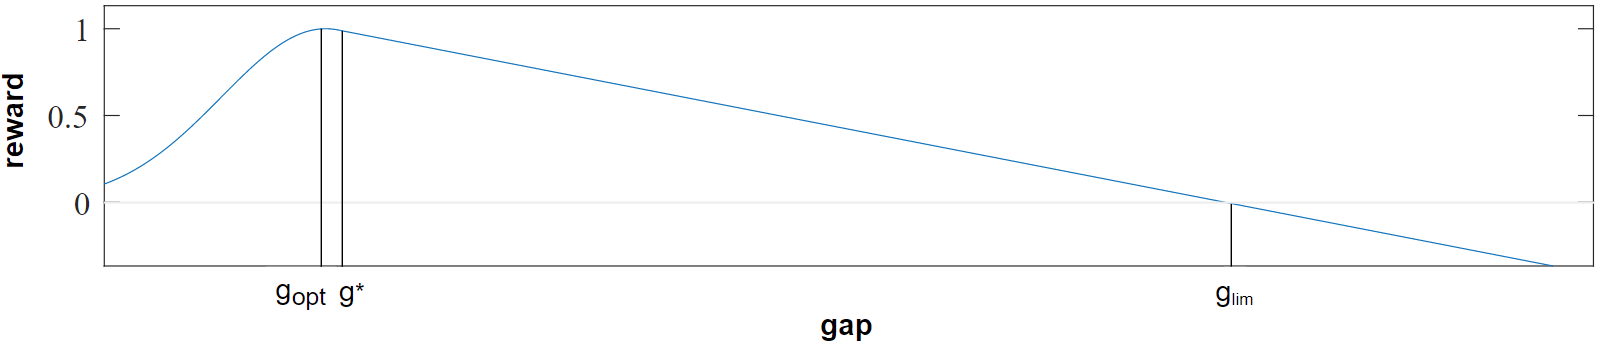
\includegraphics[width=12cm]{images/RewardFunc1}
	\caption{Factor 2 of the reward function maximizing the reward
		for car following with time gap $T$} 
	\label{fig:RewardFunc1}
\end{figure}
%
Figure \ref{fig:RewardFunc1} illustrates the reward function for
$r_2$, containing the parameter $s\sub{opt}$, $s^*$ and $s_{\rm
	lim}$. The reward function is designed in a way, that for high speeds $v$
of the following vehicle the time gap between following and leading
vehicle tends to $T$, while for low speeds the distance
between both tends to $s\sub{min}$. Different values of $T$
result in different driving styles in a way that, for lower values of
$T$ and $s\sub{min}$, the driver follows
more closely the leading vehicle resulting in a more aggressive
driving style. The results for different values of $T$ can
be found in Section \ref{sec:differentT}. Different functions for $ s
> s^*$ has been applied, but the best results regarding a smooth and
comfortable approaching of the following vehicle has been reached with
a linear function. Also, a high value of $T\sub{lim}$ results in an
early deceleration and comfortable approaching.



The third factor of the reward function aims to reduce the jerk in
order to achieve comfortable driving and has been designed analogously to the Free-Driving-Policy, 
\begin{equation}
r_3 = -\left(\frac{1}{\dot{a}\sub{comf}} \ \dv{a}{t}\right)^2.
\end{equation}
%
The contribution of the final reward function~\eqref{Rt}  at simulation time step $t$ is the weighted
sum of these factors according to
\begin{equation}
\label{rt2}
%r_t = 0.6r_1 + 1.1r_2 + 0.001 r_3 + r_4,
r_t = r_1 + w\sub{gap}r_2+w\sub{jerk}r_3,
\end{equation}
where all the factors are evaluated at time step $t$. The weights (cf.
Table~\ref{tab:agentParameters}) have been found experimentally and
can be optimized in future studies.





\subsection{Training environment}
The training environment is modeled by a leader and a follower vehicle. Both vehicles implement the point-mass kinematic model described in Section~\ref{training_environment1}. While the follower vehicle is controlled by the RL agent, the  leading trajectory is based on an AR(1) process, whose parameters
reflect the kinematics of real leaders. The AR(1) process describes
the speed of the leading vehicle and is defined as 

\begin{equation} \label{eq:AR1}
v_l(t) = c+\phi v_l(t-1)+ \epsilon_t
\end{equation}
with
\begin{equation}
E(\epsilon_t) = 0, \ \text{Var}(\epsilon_t) = \sigma, \ 
\text{Cov}(\epsilon_t\epsilon_{t+k})=0 \text{ for }k\neq 0
\end{equation}

After reaching stationarity, this process has 
\begin{equation}
\label{eq:E_AR1}
\text{the expectation value }E(v_l) = \frac{c}{1-\phi}, 
\end{equation}

\begin{equation}
\label{eq:V_AR1}
\text{the variance }\text{Var}(v_l) = \frac{\sigma^2}{1-\phi^2}, 
\end{equation}

\begin{equation}
\label{eq:ACF_AR1}
\text{the autocorrelation  }\text{ACF}(dt) = \phi^{dt}, 
\end{equation}

\begin{equation}
\label{eq:tau_AR1}
\text{and the correlation time  }\tau = -\frac{1}{\ln \phi}, 
\end{equation}
 
To adjust the parameters of the AR(1) process, typical values for real leader trajectories has to be defined: With $v_{l,des}$ as the desired speed for the leader, the mean of the AR(1) process is set to be $v_{l,des}/2$ and the standard deviation is set to be $v_{l,des}/2$. The acceleration $a\sub{phys}$ corresponds to typical physical leader accelerations. With these values and by using Equation \eqref{eq:E_AR1} - \eqref{eq:tau_AR1}, the parameters of the AR(1) process can be calculated as:

\begin{equation}
\phi = e^{(\frac{-2da\sub{phys}}{v_{l,des}})},
\end{equation}

\begin{equation}
c=(1-\phi)\frac{v_{l,des}}{2},
\end{equation}

\begin{equation}
\sigma^2=(1-\phi^2)\frac{v_{l,des}^2}{4}.
\end{equation}
The assumed typical values for $v_{l,des}$ and  $a\sub{phys}$ as well as the resulting values of the AR(1) process parameters can be found in Table \ref{tab:AR1Parameters}.
%
\begin{table}
	\caption{Assumed typical values for leading trajectories and
		the resulting values of the AR(1) process parameters for an
		update time step of \unit[100]{ms}} 
	\label{tab:AR1Parameters} 
	\begin{center}
		\begin{tabular}{ p{0.1\textwidth} p{0.1\textwidth} |p{0.1\textwidth} p{0.1\textwidth}  }
			\multicolumn{2}{c|}{Real trajectory} & \multicolumn{2}{c}{AR(1) process}   \\ \hline
			$v_{l,des}$ &$\unit[15]{m/s}$ &$\phi$ & $0.9868$\\
			$a\sub{phys}$ &$\unit[1]{m/s^2}$ &$c$ & $\unit[0.0993]{m/s}$\\
			& & $\sigma^2$ & $\unit[1.475]{m^2/s^2}$
			
		\end{tabular}
	\end{center}
\end{table}
%
Figure \ref{fig:AR1process} shows an example trajectory of the leading vehicle based on the AR(1) process using the parameters of Table \ref{tab:AR1Parameters}. If the speed exceeds the defined range of $[0, v_{l,des}]$, it is manually set to the range limits.
\begin{figure}
	\centering
	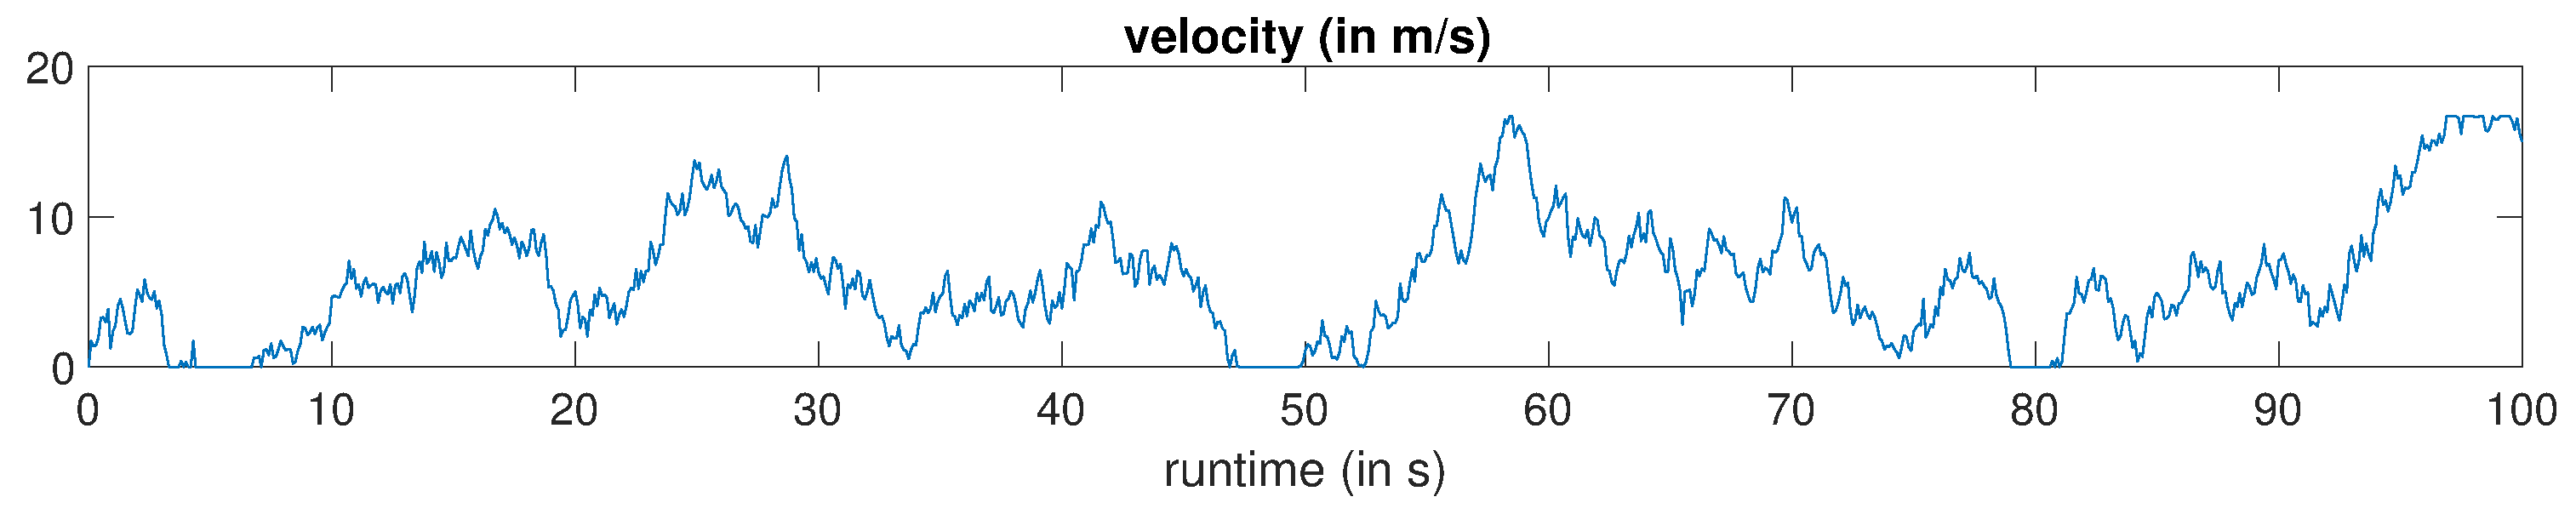
\includegraphics[width=0.95\textwidth]{images/AR1process}
	\caption{Example of a leading trajectory based on the parametrized AR1 process used to train the RL agent}
	\label{fig:AR1process}
\end{figure}
%
%\begin{figure}
%	\centering
%	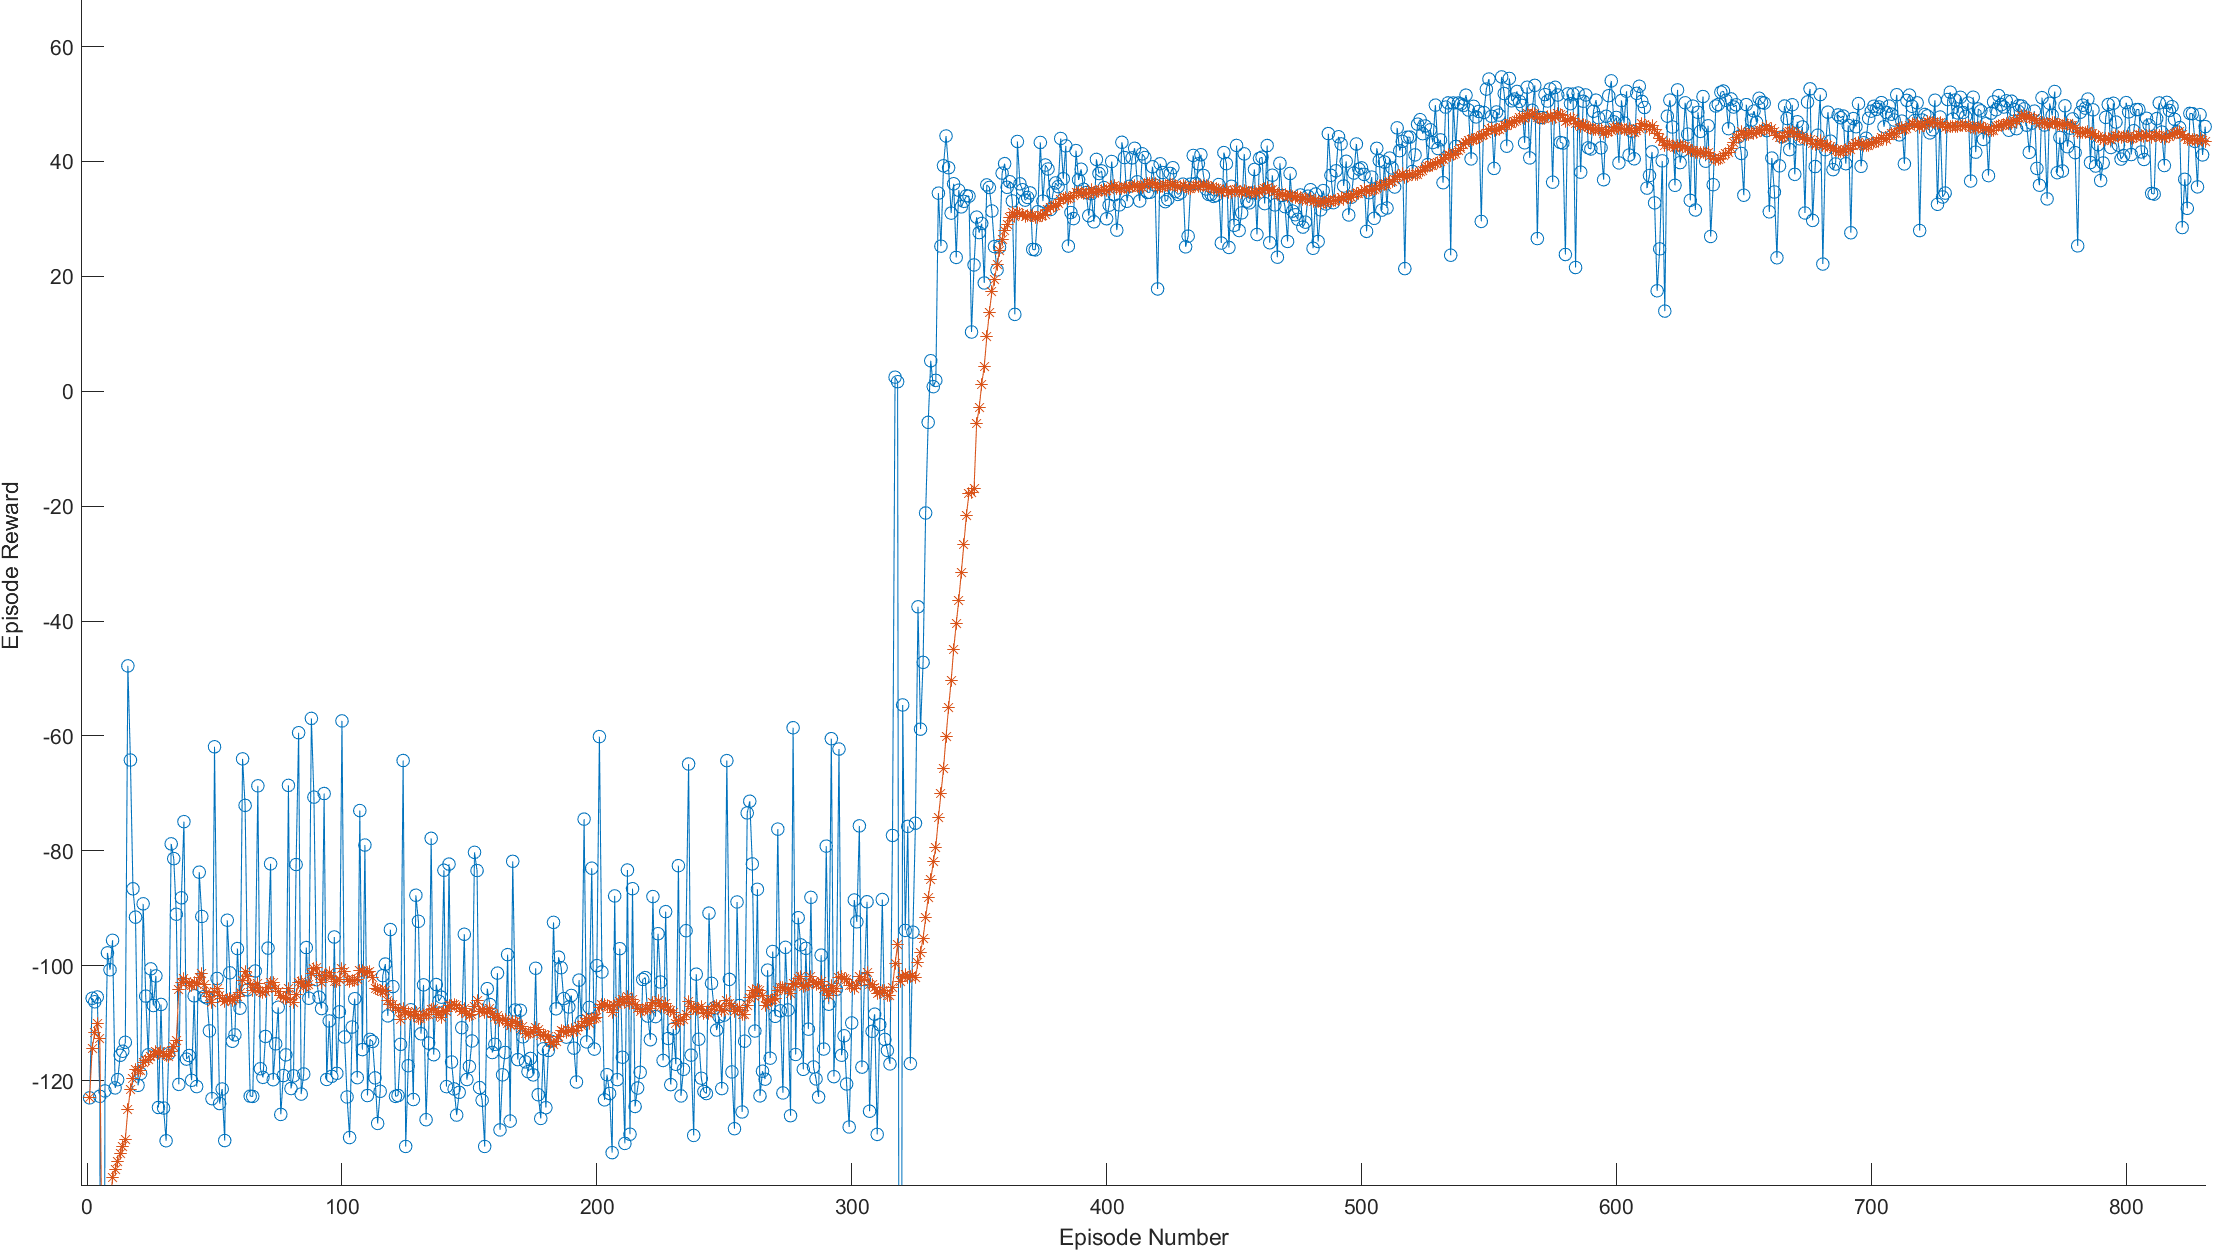
\includegraphics[width=0.95\textwidth]{images/Training}
%	\caption{RL training process, one episode contains 500
%		steps. Shown are the reward values of the individual
%		episodes (blue) and a 30-step asymmetric moving average.}
%	\label{fig:training}
%\end{figure}
%
%
One episode has a simulation time of \unit[50]{s} with a step size of
$d=\unit[100]{ms}$ resulting in an episode length of $500$
steps. The initial speeds of the following and leading vehicles are
randomly set in the range $[0,v\sub{des}]$ and $[0,v_{l,des}]$,
respectively. The initial space gap between both is set to \unit[120]{m}. 

\subsection{RL hyperparameters}
Both neural networks, Critic and Actor, are feed-forward neural networks with two layers of hidden neurons, containing 32 neurons each layer (see Figure \ref{fig:MRL}). ReLU activation functions are used. We used the same Ornstein-Uhlenbeck model as we used for the Free-Driving-Policy.
All DDPG parameters are presented in Table \ref{tab:DDPGparameters}.


%\subsection{Results of the RL training process}
%
%Figure \ref{fig:training} shows an example of the training
%process. The red line shows an asymmetric moving average reward of the last 30
%episodes. After approximately 570 episodes, the maximum
%average reward has been reached. Once the saturation has been
%confirmed at an episode count of 850, the learning
%process has been stopped.








\section{Validation}

The goal is not to minimize some error measure as in usual
calibration/validation but to check if the driving style is safe,
effective, and comfortable. The RL strategy is evaluated with respect to these metrics in different driving scenarios, described in the following.

\subsection{Response to an external leading vehicle speed profile}
The first scenario is designed in order to evaluate the transition between free driving and car-following as well as the follower's behavior in safety-critical situations. 
Figure \ref{fig:manipulatedLeader} shows a driving scenario with an
artificial external profile for the leading vehicle speed. The initial
gap between 
follower and leader is 200 meters, which refers to a free driving
scenario. The follower accelerates with $a\sub{max} = 2m/s^2$ until
the desired speed $v\sub{des} = \unit[15]{m/s} $ is reached and approaches
the standing leading vehicle. When the gap between both drops below 90
meters, the follower starts to decelerate with a maximum
  deceleration of approximately $b_{\rm
  comf} = \unit[2]{m/s^2}$ (transition between free driving and car-following)
and comes to a standstill with a final gap of approximately 
$s\sub{min} = \unit[2]{m}$. Afterwards ($t=\unit[30]{s}$),  the leading vehicle accelerates to a speed
that is below the desired speed of the follower before performing a
maximum braking maneuver ($a=\unit[-9]{m/s^2}$) to a full stop ($t=\unit[46]{s}$). At the time of the start of the
  emergency braking, the follower has nearly reached a steady
  following mode at the desired space gap $s=s_0+v_l T$. While this
  gap makes it impossible to keep the deceleration in the comfortable
  range without a rear-end collision, the follower makes the best of
  the situation by braking smoothly with a maximum deceleration of $-a
  \approx \unit[5]{m/s^2}$.  The transition between different
accelerations happens in a comfortable way reducing the resulting
jerk. Only at the beginning ($t=\unit[46]{s}$) where the situation is
really critical, the jerk $\text{d}a/\text{d}t$ exceeds the comfortable range 
$\pm \unit[1.5]{m/s^3}$. Afterwards, the leader performs a series of
non-critical acceleration and deceleration maneuvers and the follower
tries to follow the leader at the speed dependent desired space gap
$s_0+v_lT$ while simultaneously smoothing the leader's speed profile. After the leaders speed exceeds the desired speed of the follower at $t=\unit[88]{s}$ (transition between car-following and free driving), the follower keeps the desired speed $v\sub{des} = \unit[15]{m/s} $.



\begin{figure}
	\centering
	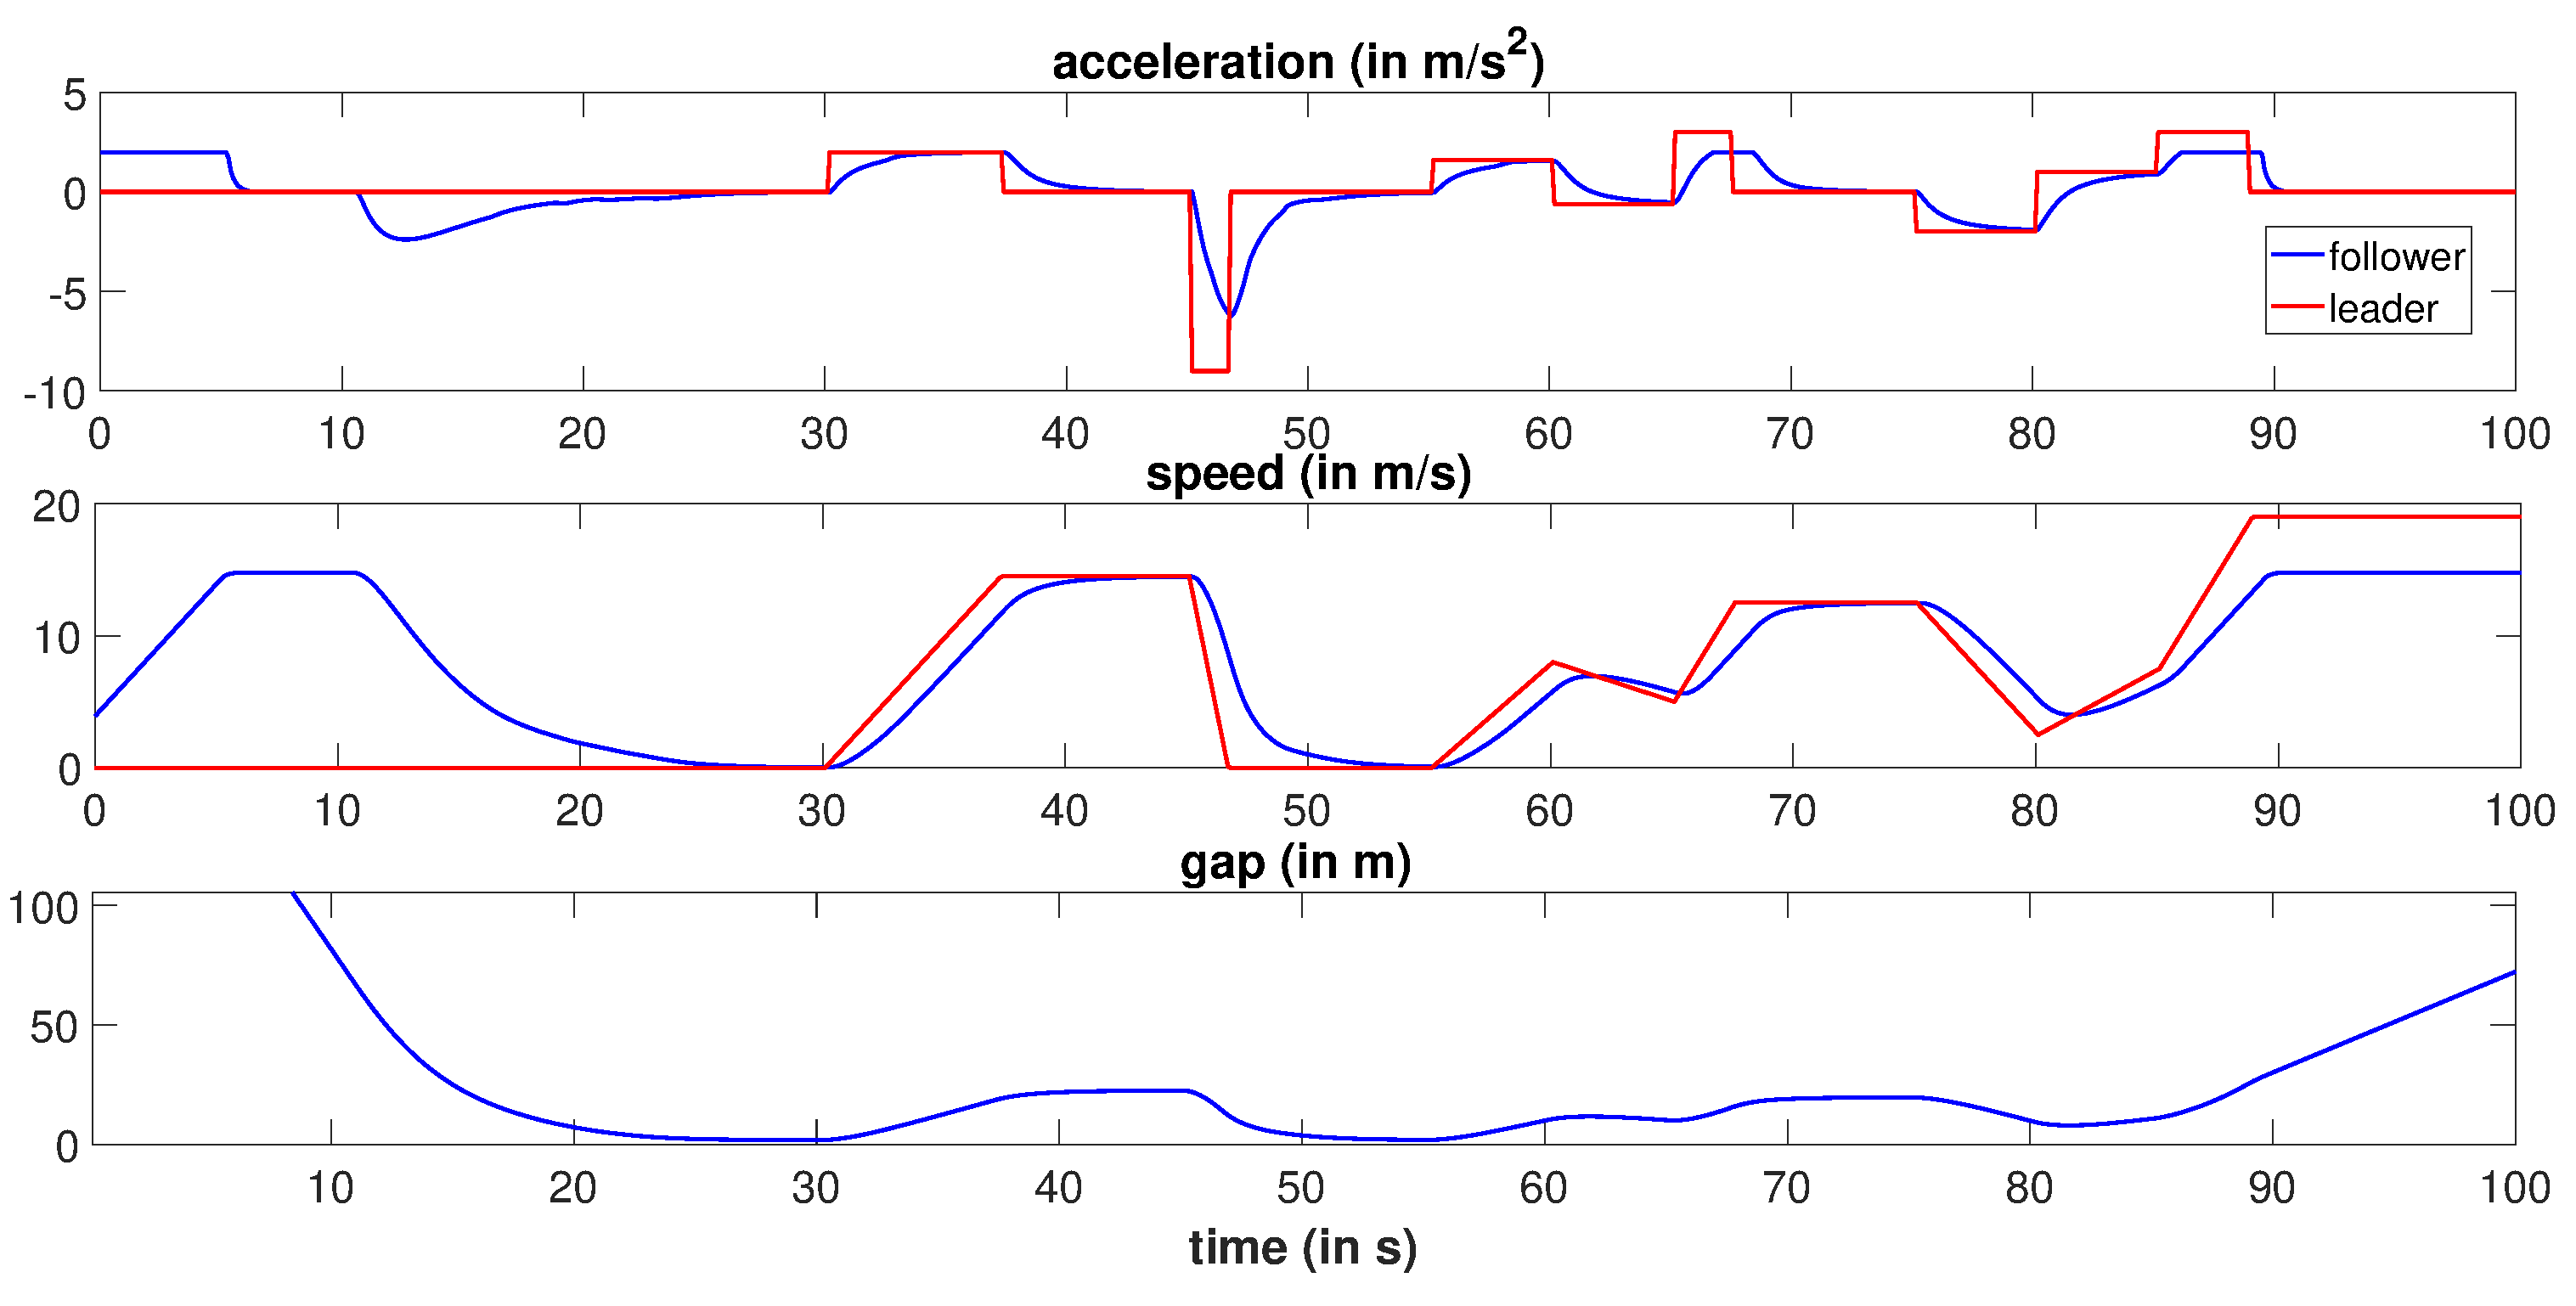
\includegraphics[width=0.95\textwidth]{images/manipulatedLeader.eps}
	\caption{Response to an external leading vehicle speed profile}
	\label{fig:manipulatedLeader}
\end{figure}

\begin{figure}
	\centering
	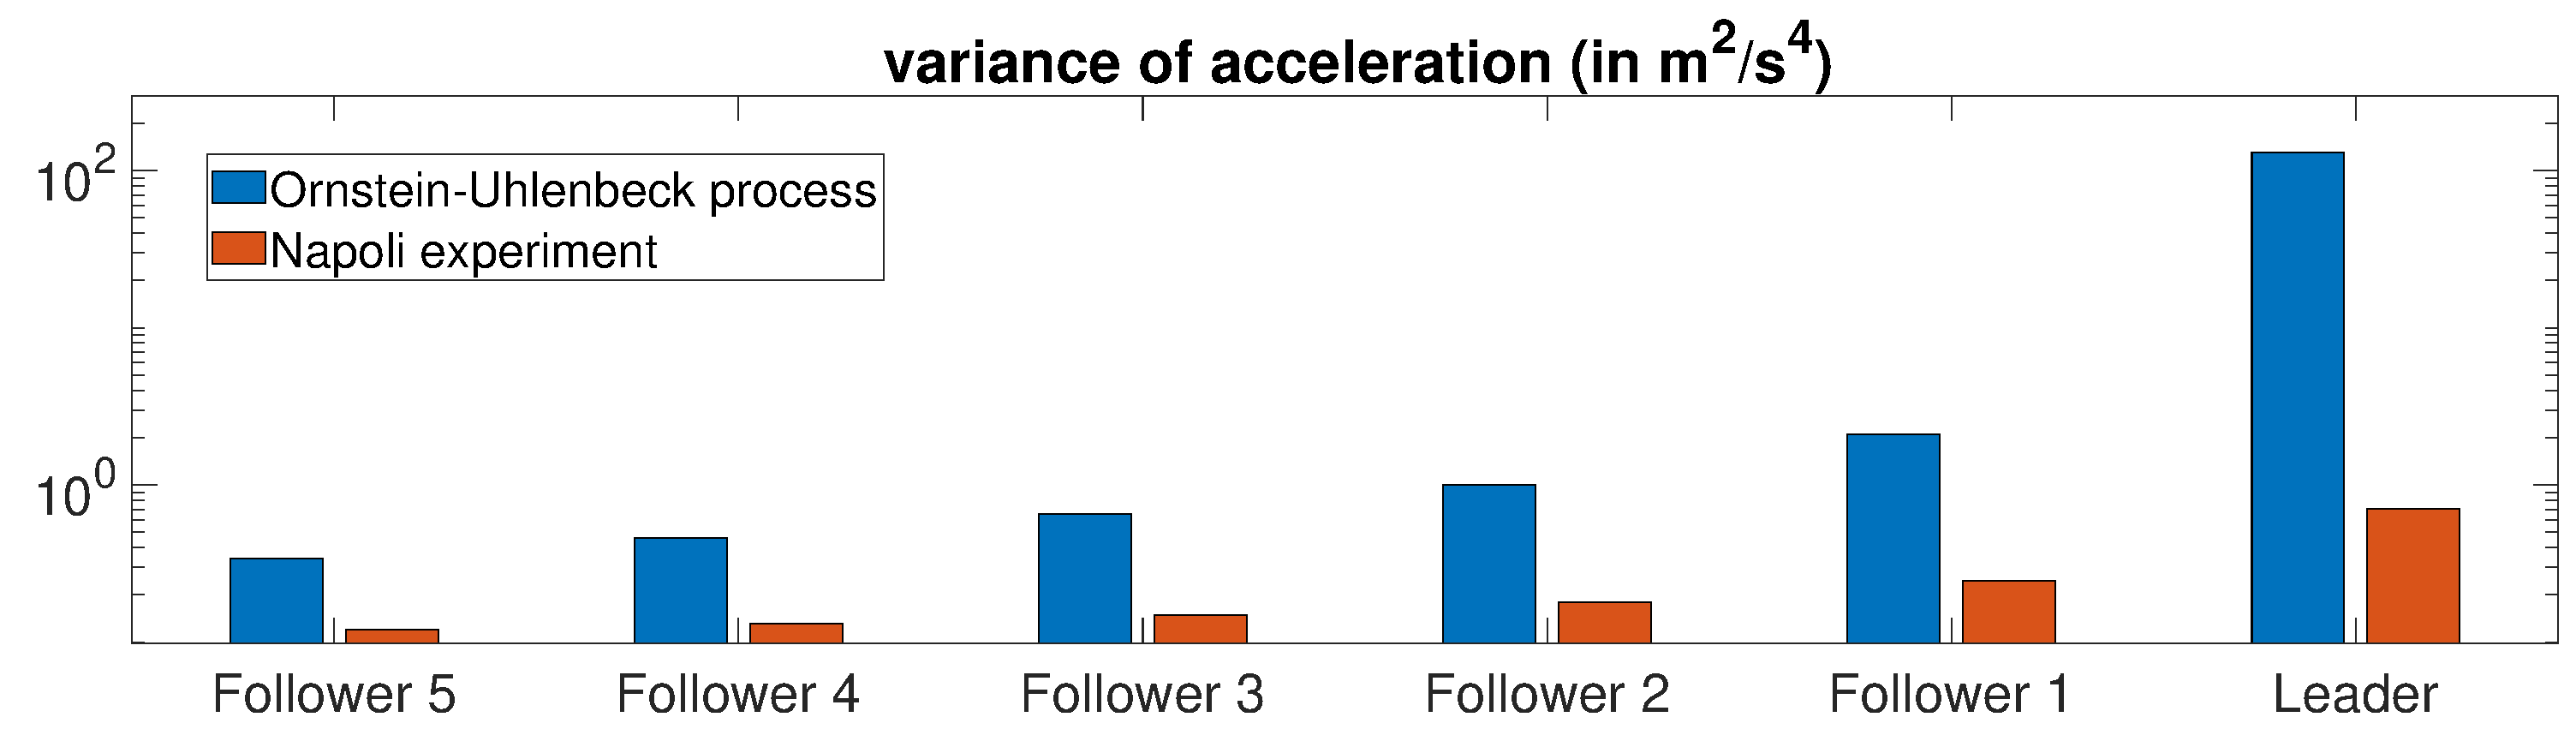
\includegraphics[width=0.95\textwidth]{images/VarAccComp}
	\caption{Comparison of the acceleration variance between
          leader and follower for a leader controlled by AR(1) (blue
          bars) and the leading vehicle of the Napoli experiment
          (red).}
	\label{fig:VarAccComp}
\end{figure}






\subsection{String stability}
\label{sec:stringStability}
The second validation scenario, shown in Figure
\ref{fig:AR1Kolonne}, consists of a leader based on the AR(1) process
that is
followed by five vehicles, each controlled by the trained RL
agent. The results show that traffic oscillations can effectively be
dampened with a sequence of trained followers, even if the leader
shows large outliers in acceleration. Figure \ref{fig:VarAccComp}
illustrates the difference of accelerations between leader and the
followers (blue bars). The last follower shows the lowest variance of
acceleration, which demonstrates the ability of the RL agent to
flatten the speed profile, to dampen oscillations and thus to increase
comfort and reduce fuel consumption and emissions.   


\begin{figure}
	\centering
	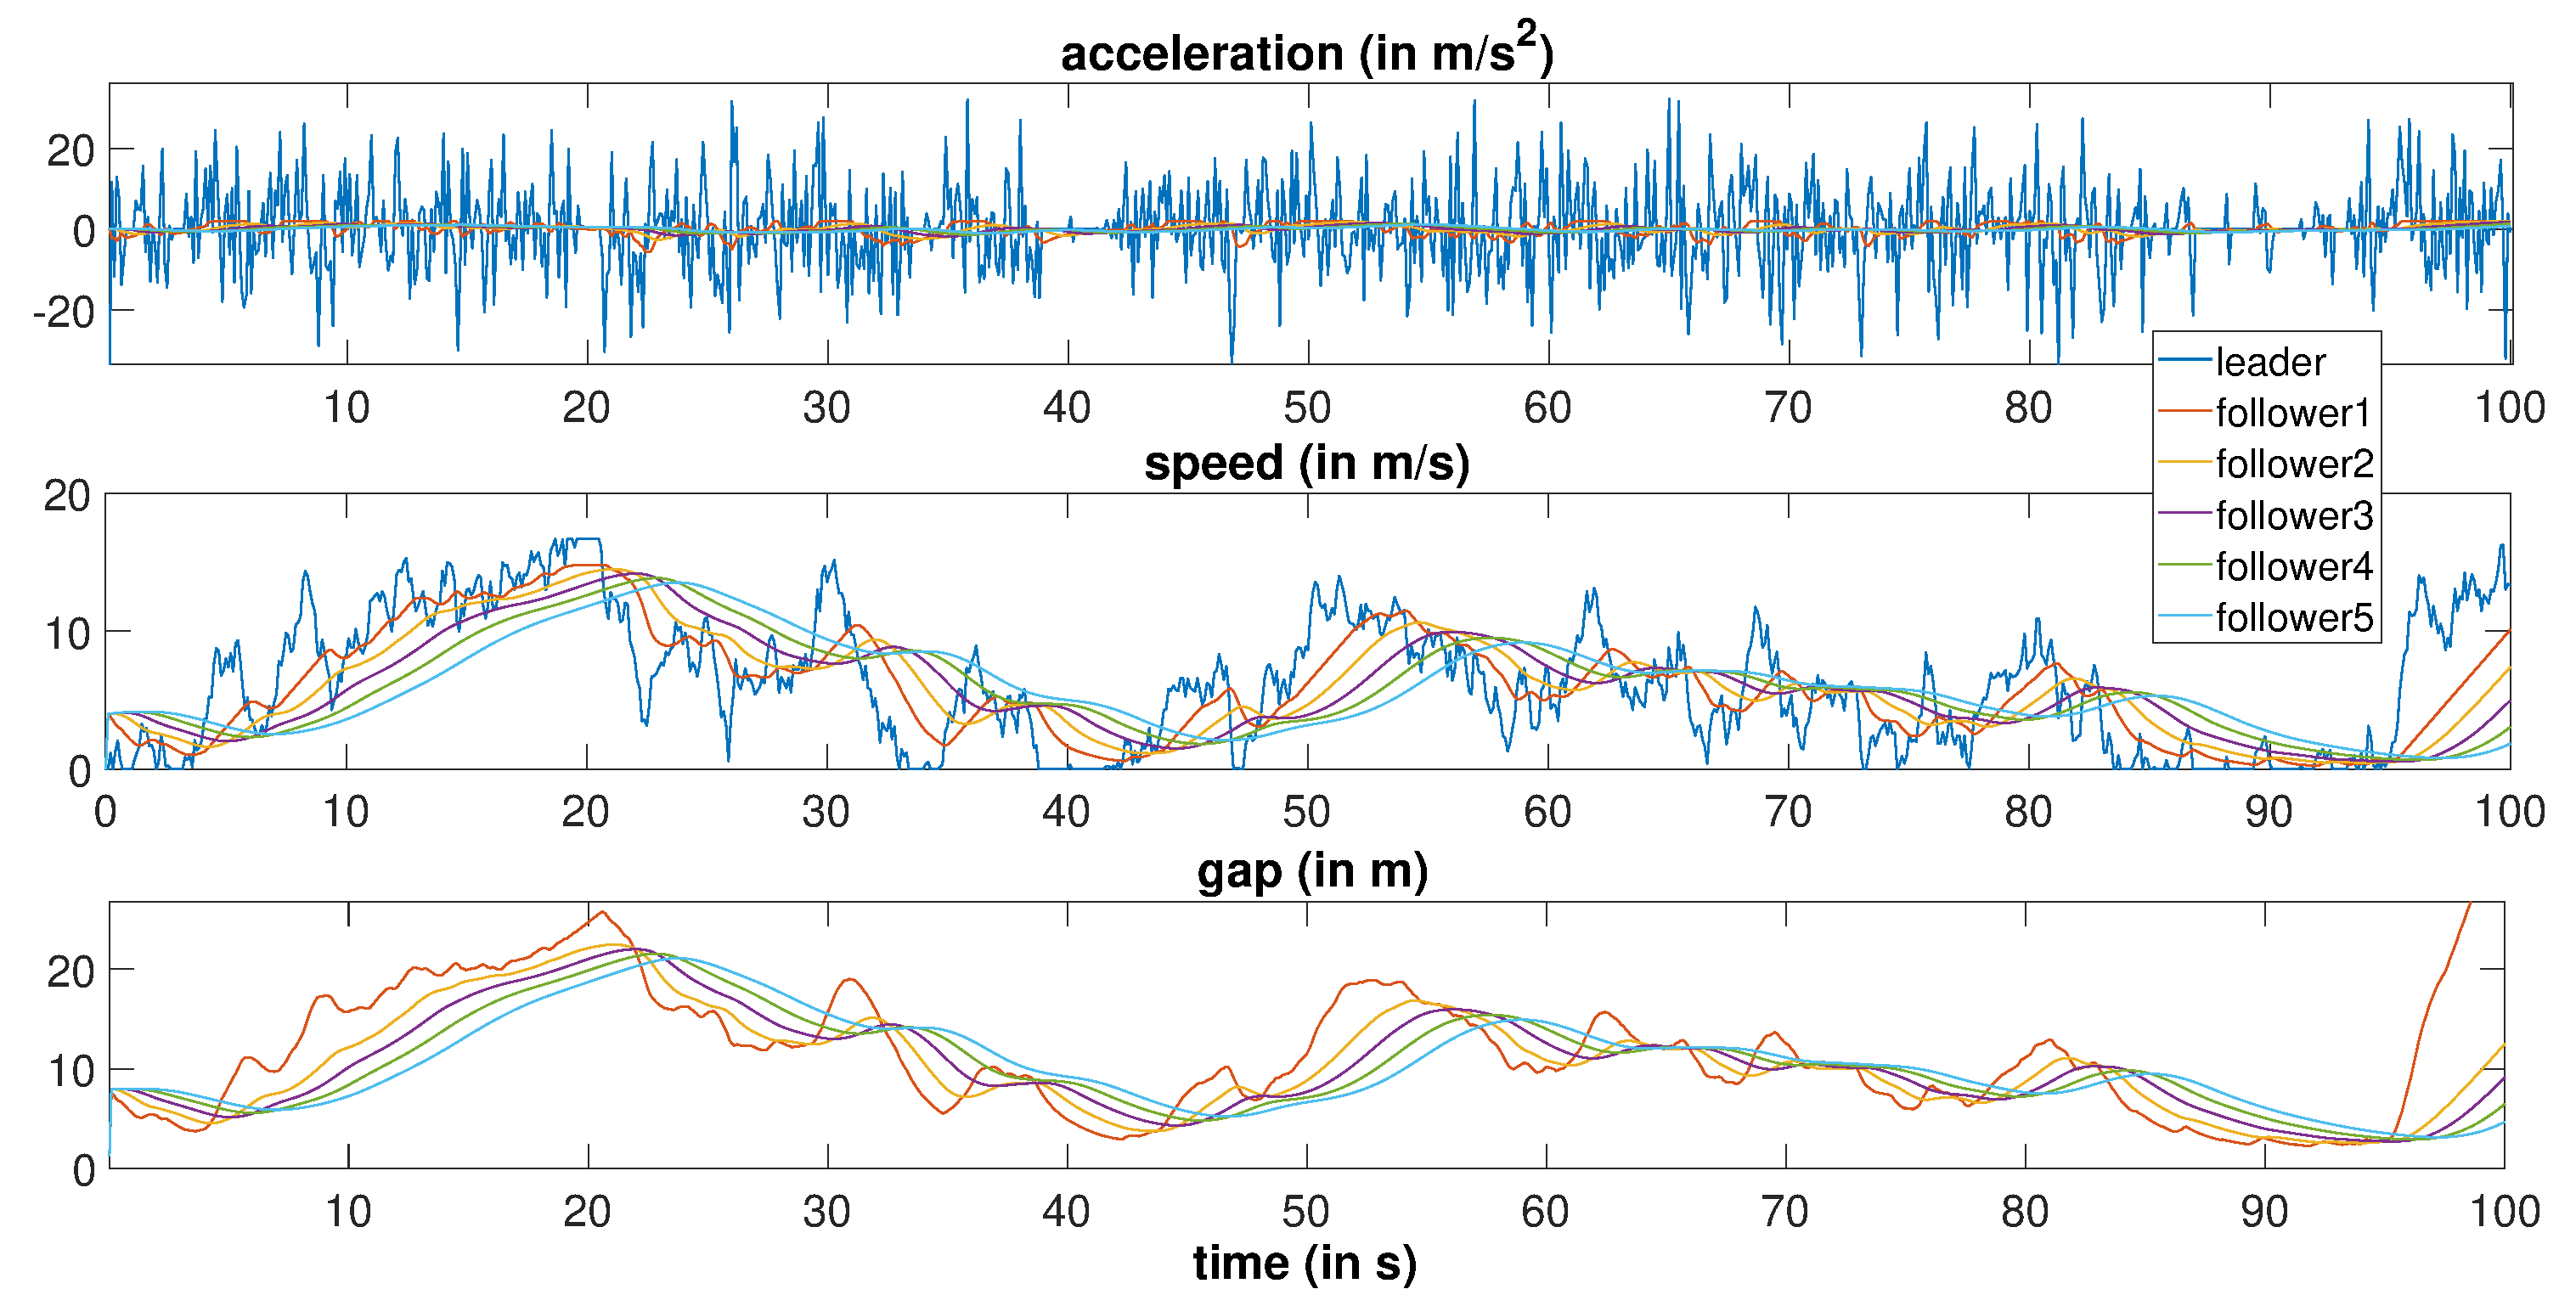
\includegraphics[width=0.95\textwidth]{images/AR1Kolonne}
	\caption{Response to a leader trajectory based on a AR(1) process}
	\label{fig:AR1Kolonne}
\end{figure}


\subsection{Response to a real leader trajectory}

In a further scenario, the abilities of the RL strategy are evaluated
with a real leader trajectory (Fig.~\ref{fig:PunzoKolonne}). This
trajectory comes from platoon driving experiments in Napoli
where high-precision distance data between the platoon
vehicles were obtained (reference to Punzo et al.). Similar to the experiment from
Section~\ref{sec:stringStability}, string stability and the reduction
of  the acceleration variance, shown by the red bars in Figure
\ref{fig:VarAccComp}, is demonstrated. At time $t = 140s$ the leader
stands still, and it can be observed, that all following vehicles are
keeping the minimum distance $s\sub{min}$ to the leader.  


\begin{figure}
	\centering
	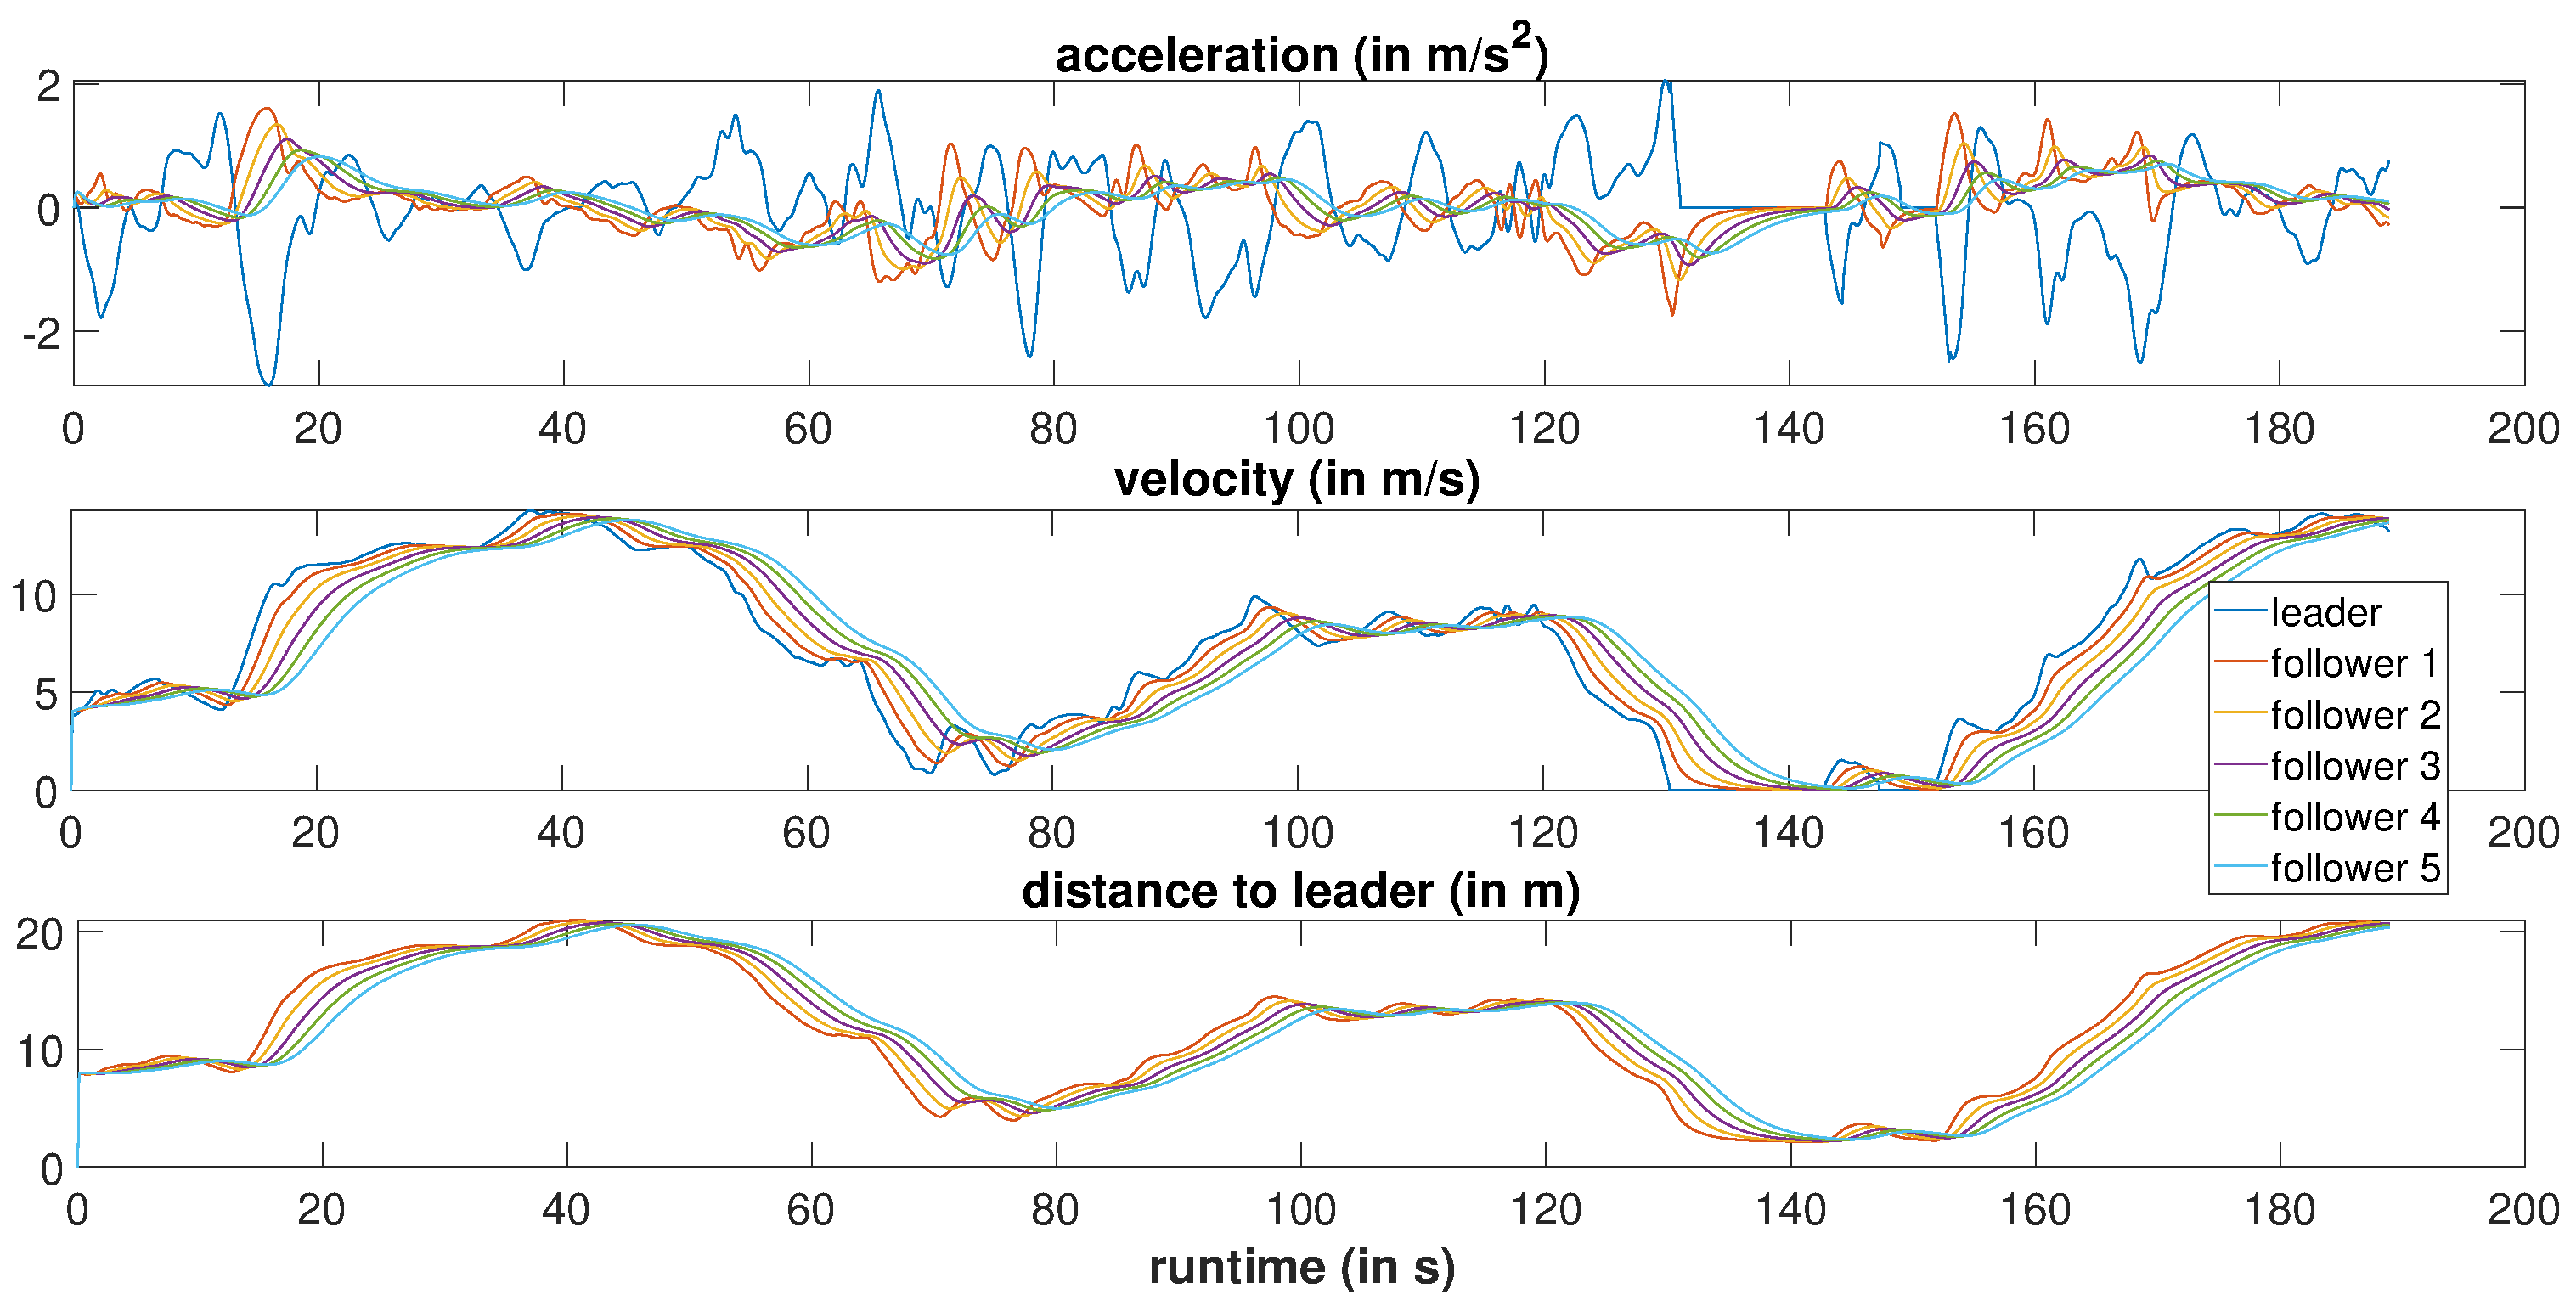
\includegraphics[width=0.95\textwidth]{images/PunzoKolonne}
	\caption{Response to a real leader trajectory}
	\label{fig:PunzoKolonne}
\end{figure}


\subsection{Response of different driver characteristics}
\label{sec:differentT}

As mentioned in Section \ref{rewardFunction}, different driving styles
can be achieved by adjusting the parameters of the reward
function. Three RL agents has been trained on a reward function, that
differs in the desired time gap $T$ between following and
leading vehicle ($T_{1} = 1.0s$, $T_{2} = 1.5s$, $T_{3} =
2.0s$). Figure \ref{fig:differentT} shows the result of these agents,
following the real leader trajectory from Napoli. It can be observed,
that a lower value for $T$ results in closer driving to the
leader which can be considered as a more ``aggressive''
driving style. Since this also means that there are less options in
increasing driving comfort without affecting safety, the follower's
accelerations and decelerations also increase although the relative
weighting $w\sub{jerk}/w\sub{gap}$ of the safety and comfort aspects in Eq.~\eqref{rt1} and \eqref{rt2} has not been
changed.

\begin{figure}
	\centering
	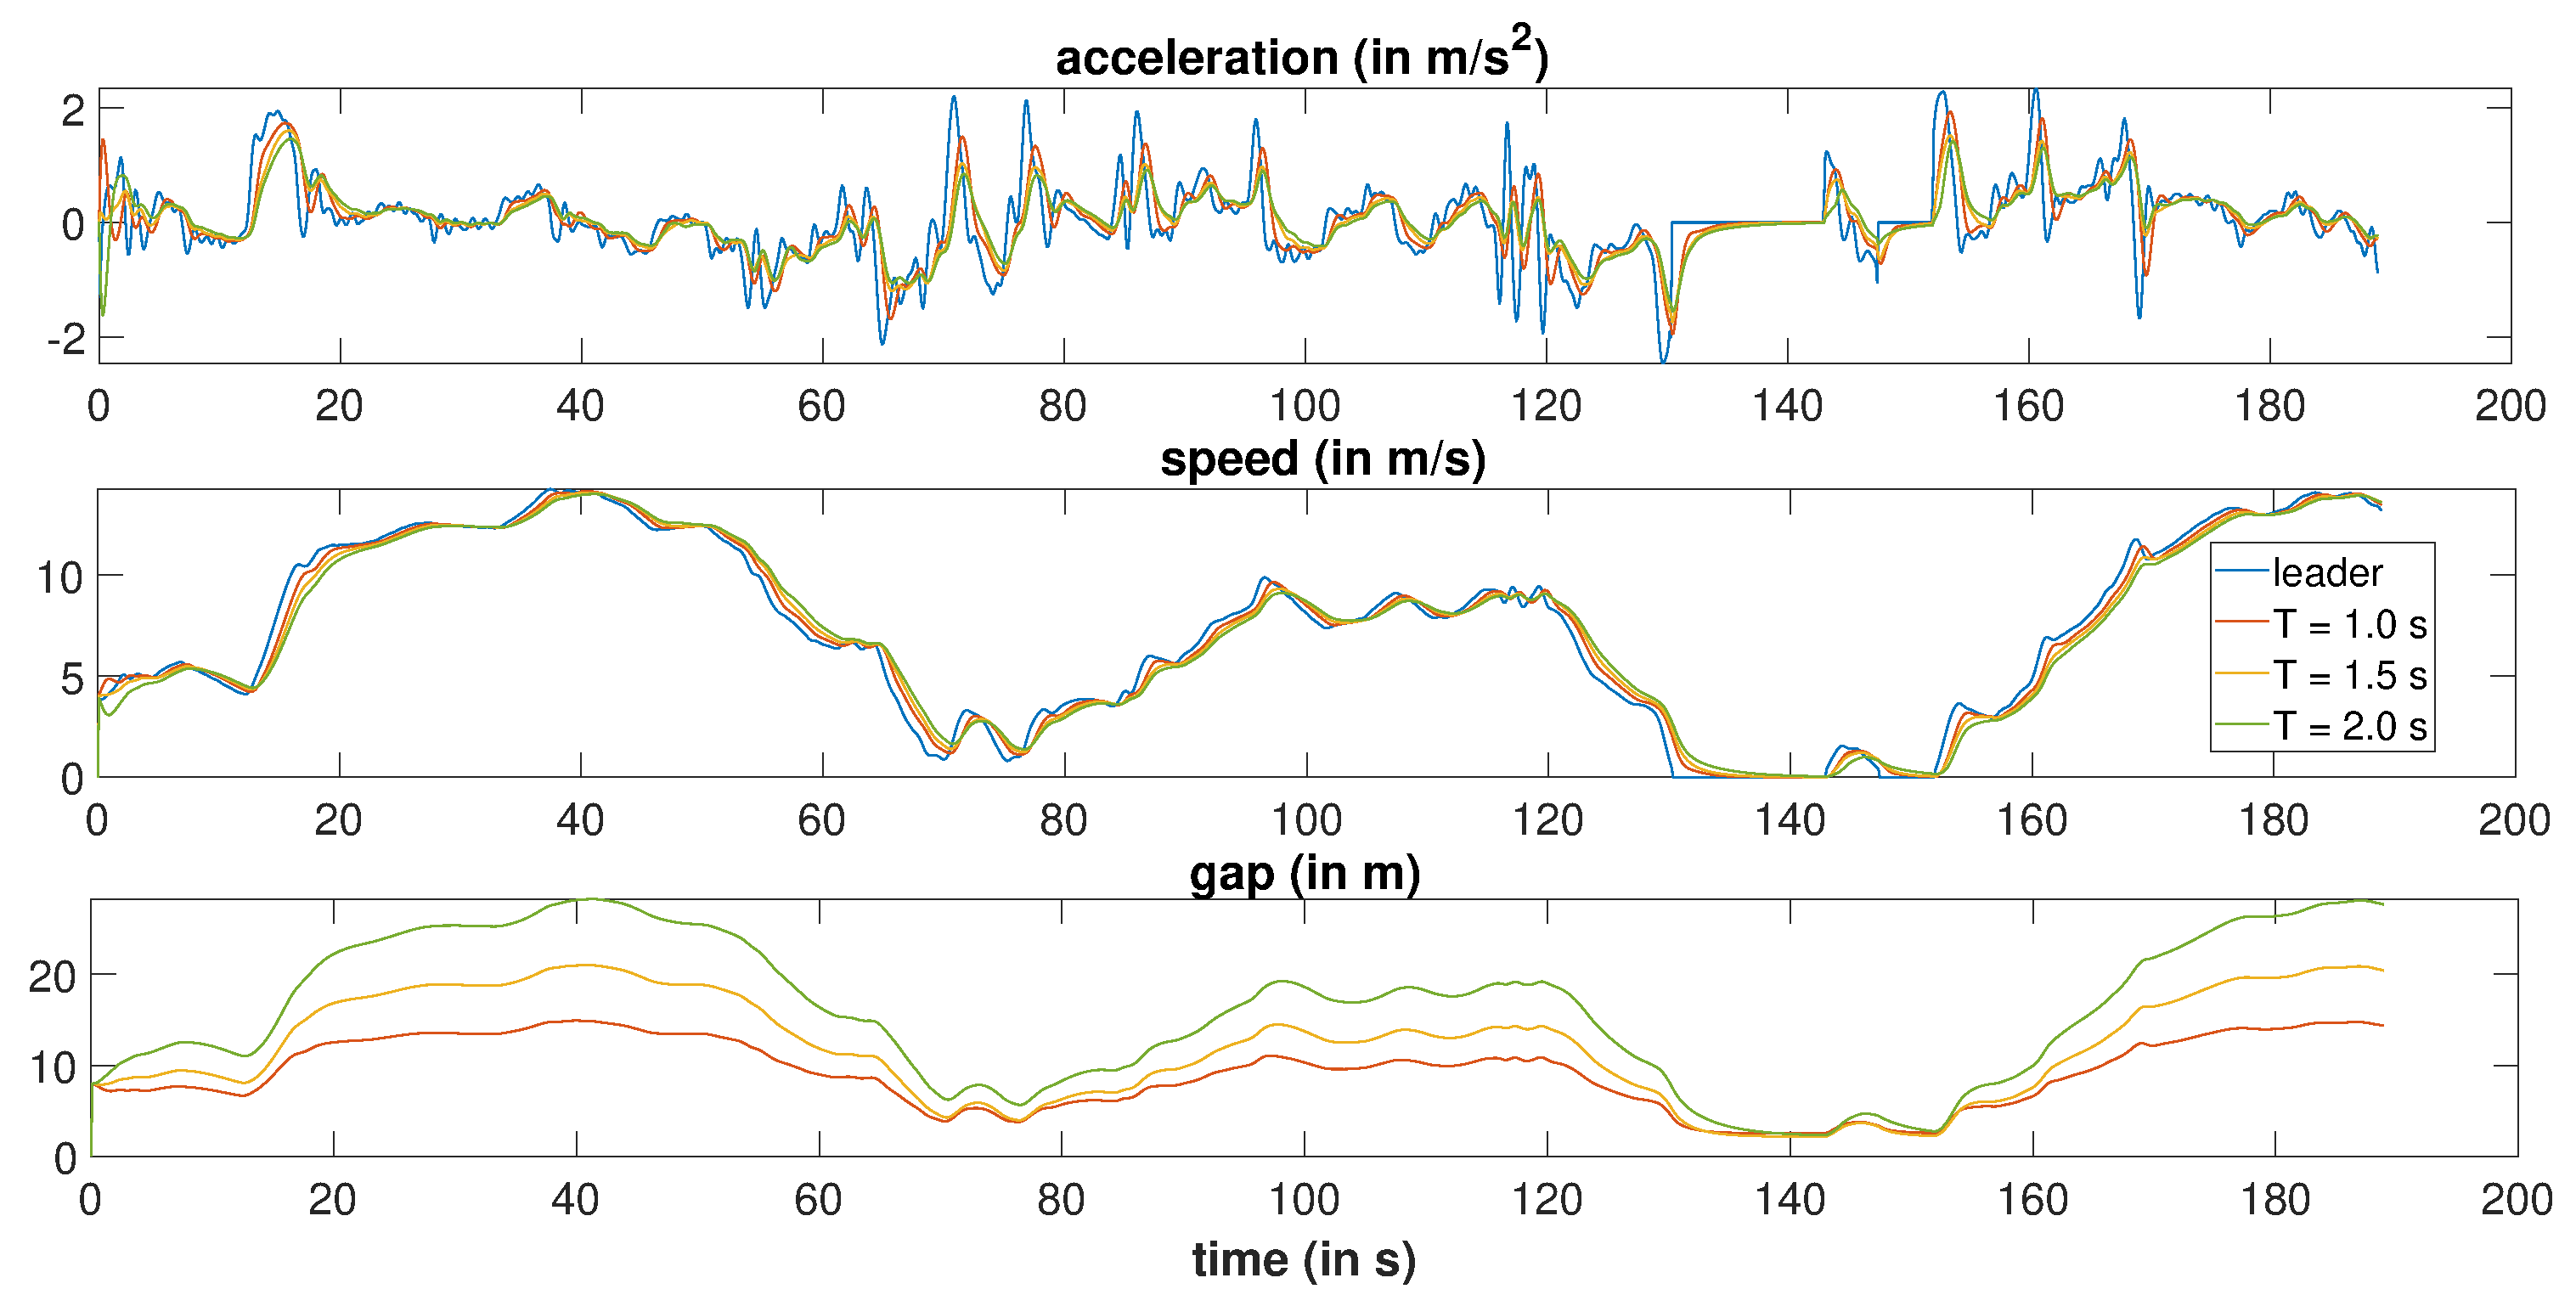
\includegraphics[width=0.95\textwidth]{images/differentT}
	\caption{Impact of differently parametrized RL agents
          on the driving behavior }
	\label{fig:differentT}
\end{figure}


\subsection{Cross validation with the Intelligent Driver Model}
To compare the performance of the RL agent with that of
classical car-following models, we chose the commonly used
Intelligent-Driver Model (IDM)\cite{Opus} whose acceleration is given
by
\begin{equation}
\label{eq:IDM}
a=a\sub{max}\left(1-\left(\frac{v}{v\sub{des}}\right)^{4}-\left(\frac{s^{*}\left(v, \Delta v\right)}{s}\right)^{2}\right),
\end{equation}
with
\begin{equation}
\label{eq:IDMsstar}
s^{*}\left(v, \Delta v\right)=s\sub{min}+\max \left(0,vT+\frac{v \Delta v(v-v_l)}{2 \sqrt{a\sub{max} b\sub{comf}}}\right).
\end{equation}
Notice that the IDM parameters desired
speed $v\sub{des}$, minimum gap $s\sub{min}$, time gap $T$, maximum
acceleration $a\sub{max}$, and
comfortable deceleration $b\sub{comf}$ are a subset of that of the RL reward
function. 

First, we calibrate the IDM on the Napoli data set by
minimizing the sum of squares of the relative gap error,
$\mathrm{SSE}(\ln s)$, of the first follower with respect to the
data (cf. Table~\ref{tab:IDMparameters}). The same parameters are also
assumed for the reward function of the RL agent before it was trained
on the artificial AR(1) generated leader speed profile. Notice that the RL agent used the Napoli data only
indirectly by parameterizing its reward function.
\begin{table}
	\caption{IDM parameters calibrated to the Napoli
            data and also used for the reward function of the RL agent}
	\label{tab:IDMparameters} 
	\begin{center}
		\begin{tabular}{ p{0.14\textwidth} |p{0.1\textwidth}  } 
		Parameter & Value   \\ \hline
			$T$ & $0.83s$\\
			$s\sub{min}$ & $4.90m$\\
			$a\sub{max}$ & $4.32m/s^2$\\
			$b\sub{comf}$ & $2.34 m/s^2$\\
			$v\sub{des}$ & $33.73m/s$
			
		\end{tabular}
	\end{center}
\end{table}

Figure \ref{fig:IDMvsRL} shows the results for: First, the RL agent, calibrated on the real follower data. Second, the IDM, calibrated on the follower data. And third, the real follower of the Napoli experiment. To evaluate the performance, for both approaches the respective objective function has been computed. The objective function of the RL agent correspondences to the reward function, while the Goodness-of-Fit Function $SSE(s)$ defines the objective function of the IDM. A comparison between RL agent and IDM for both, the reward function and the Goodness-of-Fit Function, is shown in Table \ref{tab:objectiveFunc}. For both objectives the RL agent shows a better performance.

\begin{figure}
	
	\centering
	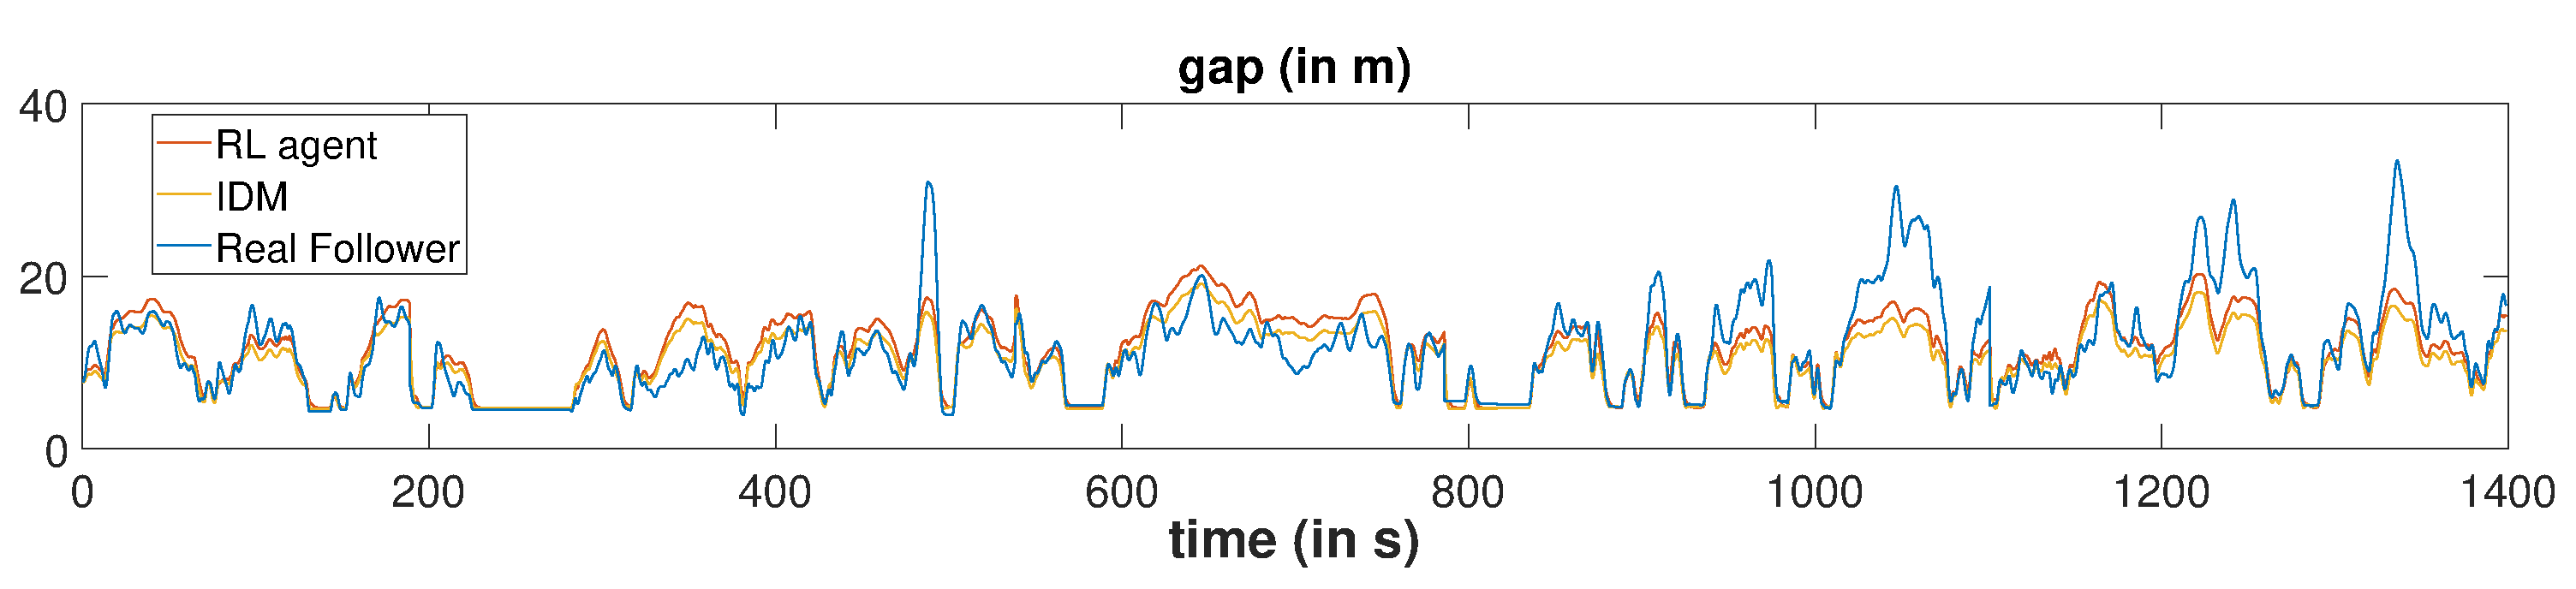
\includegraphics[width=0.95\textwidth]{images/IDMvsRL_dist}
	\caption{Comparison between IDM and RL agent, calibrated on the same set of parameters}
	\label{fig:IDMvsRL}
\end{figure}

\begin{table}
	\caption{Comparison between calibrated RL agent and IDM for accumulated Reward and Goodness-of-Fit Function $SSE(log(s))$} 
	\label{tab:objectiveFunc} 
	\begin{center}
		\begin{tabular}{p{0.3\textwidth} | p{0.2\textwidth} p{0.2\textwidth}  } 
			& RL agent & IDM   \\ \hline
			$SSE(log(s))$ & $389.10$ &  $418.05$	\\
			Accumulated Reward &  $6.86 \times 10^3$   & $6.73\times 10^3$
			
		\end{tabular}
	\end{center}
\end{table}


\section{Conclusion/Discussion}
evaluation of safety and comfort, comparison to IDM



\bibliography{RL_vehicles_references}

\end{document}
